\chapter{\label{ch:ch5-results}Results}
%3146 words
This section presents and discusses the results of our experiments based on the three models and the datasets introduced in Chapter \ref{ch:4-methods}. It also describes the rationale behind deciding which experiments should be run.

Results are given as obtained on the test set. Across all datasets and experiments, validation and test set metrics differ by less than 1\% on average. We observe no undue overfitting and unless explicitly mentioned, AUCs on the training set are generally higher by 0.02 to 0.06. 
\section{HEXEvent dataset} \label{sec:hexevent_results}
To obtain a baseline, we evaluate all three models on the HEXEvent dataset as used in \cite{dsc} and introduced in \ref{subsec:hexevent}. The results of these experiments are shown in Figure \ref{fig:hexevent_auc}.

\subsubsection{Analysis of main findings}
Generally all models perform extremely well with AUCs nearing 90\%. While differences are small, RASC seems to perform slightly better than the other models.
%They also perform very similarly, making it hard to differentiate them based on their ROC curves. The Attn model seems to perform slightly better than the other models. 

Assessing our reimplementation, we observe a small difference between the AUC value reported in \cite{dsc} (mean 0.899, standard deviation of 0.18) and the ones we observe (mean 0.873, standard deviation of 0.06). This is likely the result of random statistical noise influenced by different random seeds between runs and differences between TensorFlow/Keras (their implementation) and PyTorch (our implementation). Notably, when reevaluating the publically available original implementation in a single run, we also obtain results (0.872 AUC) closer to the results of our reimplementation. 
%There is a small (~2\%) difference in the AUC values in the AUC values for the DSC model reported in \cite{dsc} (89.9 AUC) and the ones we observe (87.1 AUC original). 
Thus, we conclude that, albeit with minor caveats, the reimplementation and replication of \cite{dsc} was successful.

\begin{figure}
	\centering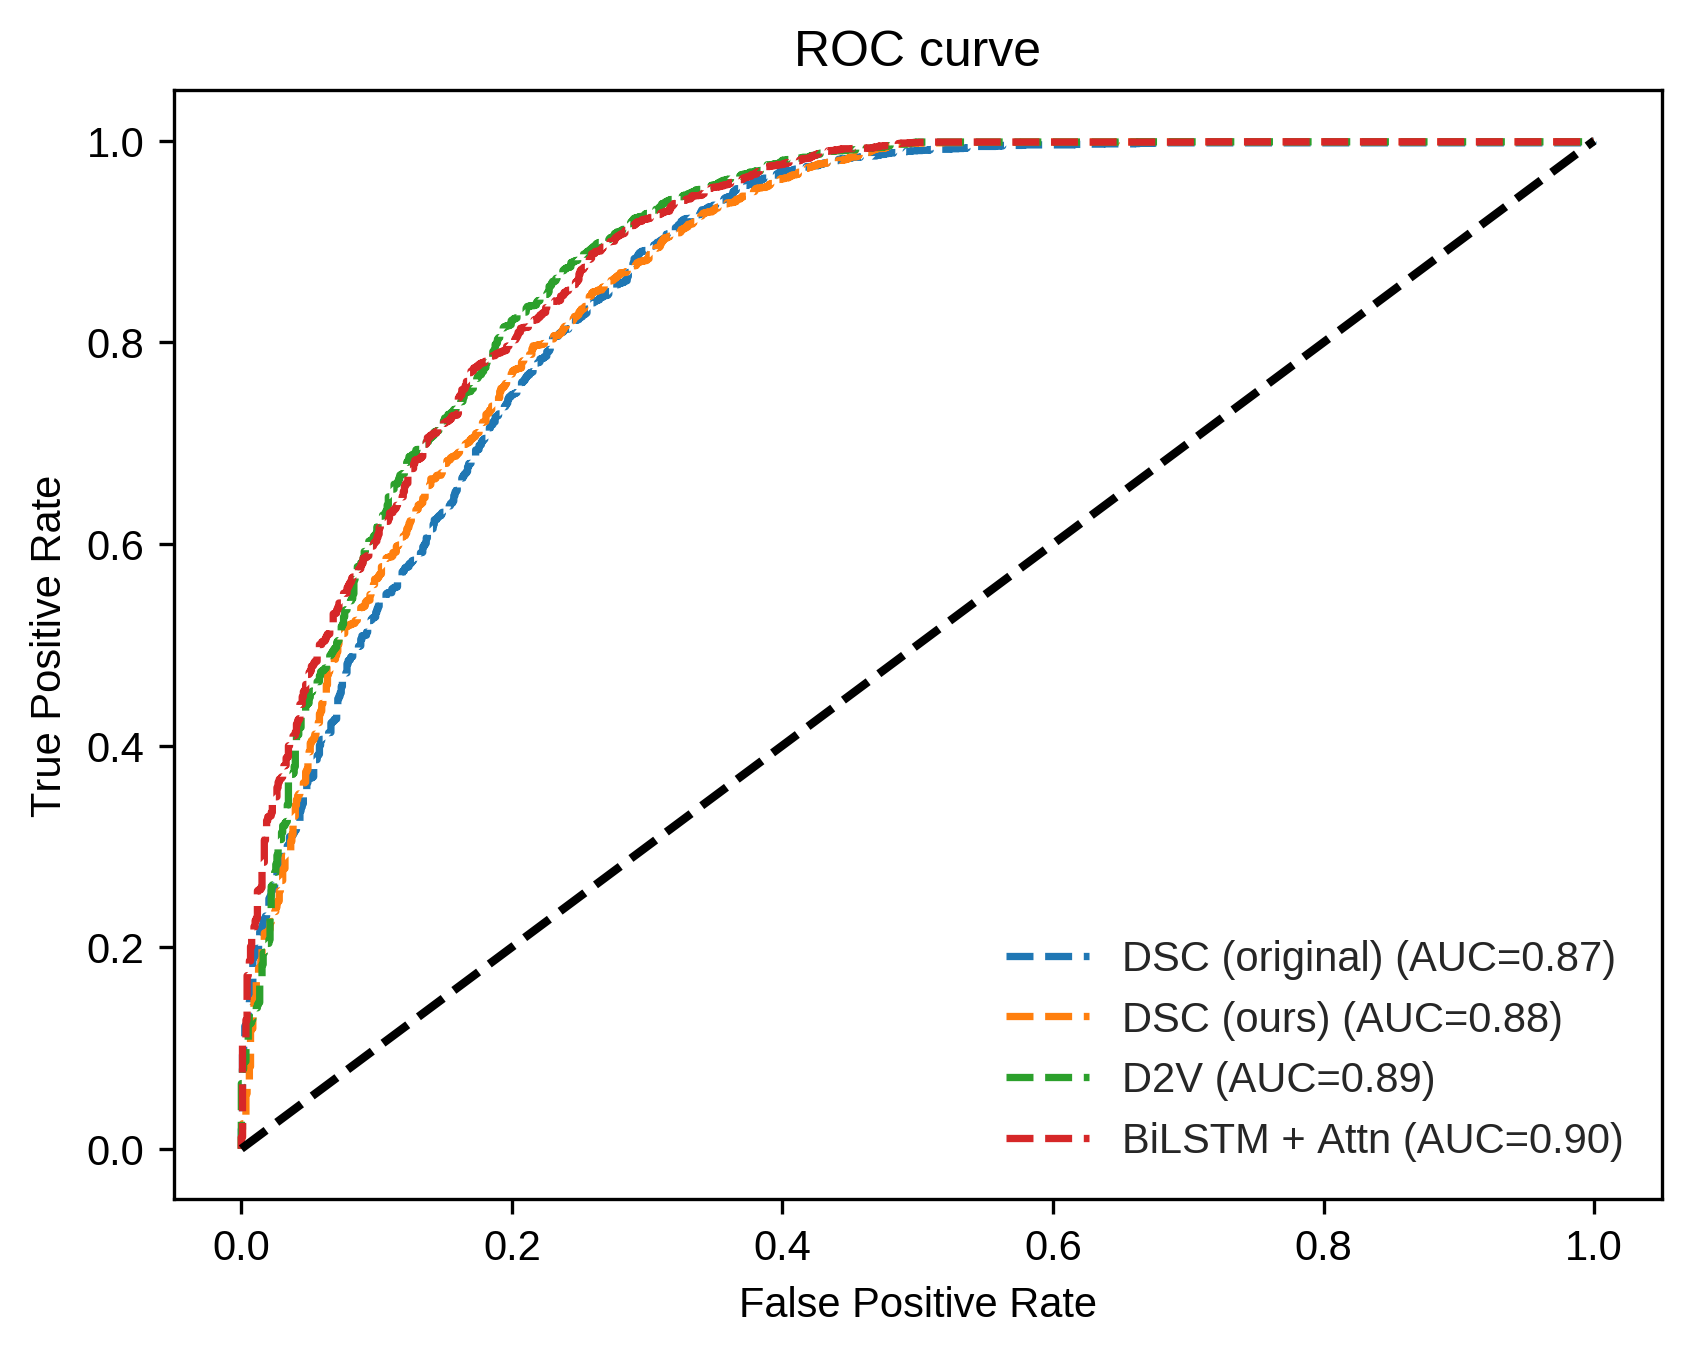
\includegraphics[width=0.7\textwidth]{../visualizations/ch5-results/hexevent_cross_model_roc_auc_comparison.png} 
	\caption{Comparison of the ROC curves of the three models as well as the original implementation on the HEXEvent dataset. The values of the original implementation were obtained by rerunning the training on the publicly available implementation. }
	\label{fig:hexevent_auc}
\end{figure}

%main takeaway: all models perform extremely well \& very similarly



%To showcase the advantage of using the attention mechanism, we also included the BiLSTM-based model where only the last output is used for classification. This model performs significantly worse than the other ones.

% Observation: Performance heavily drops when no lengths feature is used

\subsubsection{Length features are necessary}
Reimplementation was completed piece-wise, that is, first the sequence features were added as input, then the networks were trained to ensure that this was done correctly and then the length features were added. This lead to an interesting observation: model performance is significantly worse when no length features are given to the models. Quantitative results for this observation are given in Table \ref{table:results_hexevent}. This observation is true across models and leads to an average relative performance drop of over 66\%. The information about the secondary structure obtained in the lengths seems to be necessary for the models to obtain good predictive power.

% 0.684, 0.737, 0.663
%0.255, 0.282, 0.268
\begin{table}[h!]
	\centering
	\begin{tabular}{| l | c | c | c| c} 
		\hline
		Model name & Only sequences & Sequences + lengths & Relative performance improvement\\
		\hline
		DSC & 0.618 & 0.873 & 0.684\\
		D2V & 0.614 & 0.896 & 0.737\\
		BiLSTM + Attn & \textbf{0.636} & \textbf{0.904} & 0.663\\
		\hline
	\end{tabular}
	\caption{Performance of the main models on the HEXEvent dataset with and without length features given as AUC. The relative performance improvement (from adding the length features) was computed as $\frac{AUC - AUC_{no\_lengths}}{AUC - 0.5}$. Computing it this way accounts for the baseline AUC of random guessing being 0.5.
	}
	\label{table:results_hexevent}
\end{table}
%TODO: overlaps to one site
\subsubsection{Further investigations}
To further investigate, we also test three other models: MLP100, MLP20 and MLPLinear which respectively contain 100, 20 and 20 trainable parameters. The models are MLPs with one hidden layer which only take the length features as inputs. MLPLinear doesn't contain a non-linear activation function after its hidden layer.

\begin{figure}
	\centering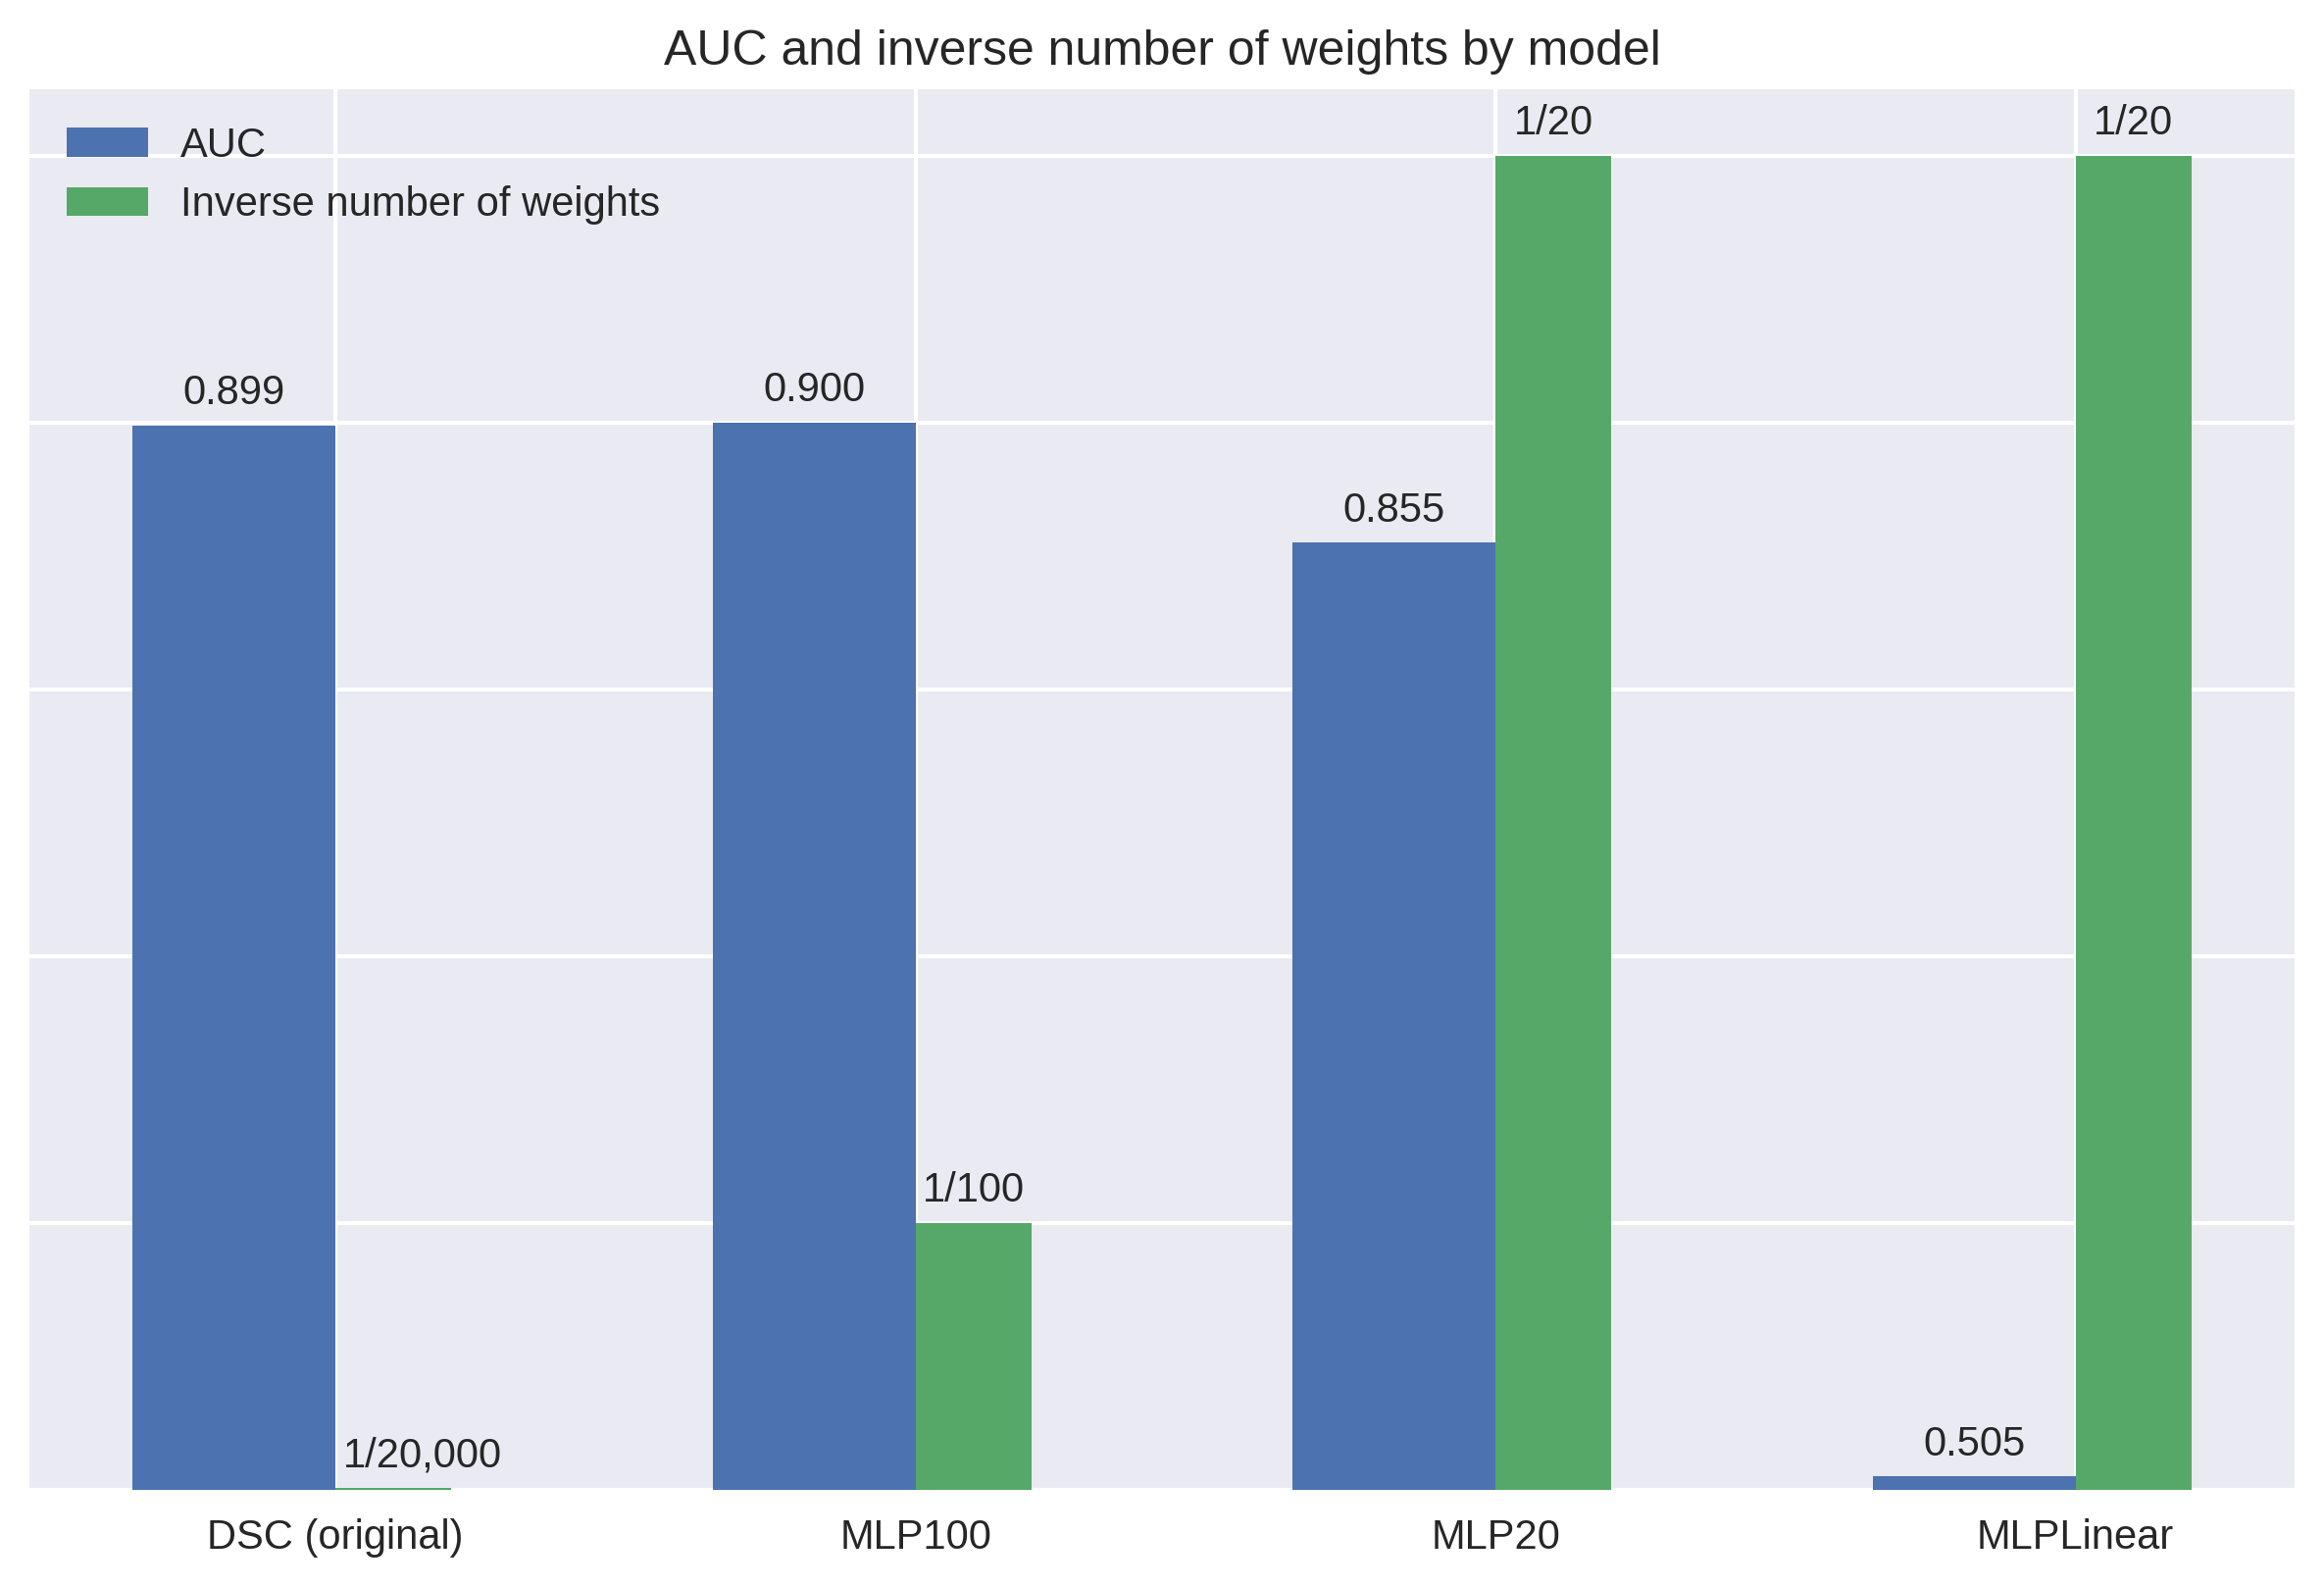
\includegraphics[width=0.85\textwidth]{../visualizations/ch5-results/dsc_funeral_barchart.png} 
	\caption{Stress testing the HEXEvent dataset used in \cite{dsc}. The graph shows the performance as well as the inverse of the respective model sizes used.}
	\label{fig:dsc_funeral}
\end{figure}

Surprisingly, the results in Figure \ref{fig:dsc_funeral} show that it is possible to replicate the results of \cite{dsc} with these very simple models using two to three orders of magnitude fewer parameters (note that DSC has 20,001 parameters). Model performance is improved by adding further parameters and breaks down when no non-linearities are used in the network. This indicates that the models capture a relatively simple, but non-linear relationship between the lengths and the classification of an exon in the dataset. 
There are multiple possible explanations for why this is:
\begin{enumerate}
	\item There are confounders in the dataset learned by the model. As discussed in Section \ref{subsec:hexevent}, EST-based data is inherently biased. The biases inherent in EST-based data could be captured by the exon and intron structure and the model is learning to make its prediction based on this bias. 
%	This explanation is made more likely, if the findings on the HEXEvent dataset don't replicate on the other datasets we evaluate.
	\item Exon splicing is extremely well predictable based on the lengths of neighbouring introns and exons. This is very unlikely given that research into splicing has been ongoing for over 40 years. 
%	This explanation, albeit unlikely already, can be disproven if this observation fails to replicate on other datasets.
	\item There are bugs (e.g. mixing of testing and validation data) in our reimplementation. In the first instance, this is unlikely given that we were able to replicate the original results of \cite{dsc}. To reduce complexity and further reduce the likelihood of a bug leading to these observations, we extracted the complete code for replicating the results of the simple MLP models from \ref{fig:dsc_funeral} into a single file. Additionally, in case of a data leakage bug, the performance of the linear model likely wouldn't break down either. Therefore, we judge bugs in our reimplementation unlikely.
\end{enumerate}

Overall, we conclude that the HEXEvent-based dataset is most likely fundamentally flawed and suffers from confounders.
These findings have strong implications. It calls into questions the meaningfulness of \cite{dsc}'s results, showing the competitiveness of their model. These findings likely also warrant a critical investigation of any other conclusions drawn from papers based on the HEXEvent database. At the time of writing, the HEXEvent paper is cited 34 times. While most of these citations are in passing, multiple papers use a HEXEvent-derived dataset for the training of Machine Learning models such as SVMs \cite{buschhertel}, Random Forests \cite{flawed4} \cite{flawed1}, Decision Trees \cite{flawed2} or AdaBoost-based algorithms \cite{flawed3}. The validity of these papers results' are called into question by these findings.

These data quality issues motivated us to construct alternative, better, datasets. We now give their results.


% many of them, even correlational studies, say that this is a feature, rather than a bug
% how true is this?
% mgith even have to post-pone condemning of HEXEvent dataset until I find a better one 

%Recognition of alternatively spliced cassette exons based on a hybrid model -- confirmed

%A classification of alternatively spliced cassette exons using AdaBoost-based algorithm -- actually says that this is a feature, not a bug

%G2P: Using machine learning to understand and predict genes causing rare neurological disorders --- definitely in some capacity
%Exon size and sequence conservation improves identification of splice-altering nucleotides -- this observation is actually their main contribution
% short exons are more likely to be alternatively spliced


%We showed that the EST-based HEXEvent dataset is likely too flawed to serve as a basis for our methods. Thus, we try to construct an alternative dataset.




%TODO: tSNE of MLP embeddings?


\section{GTEx-based datasets} \label{sec:gtex}
\subsection{Exon-centric datasets} \label{subsec:gtex_exon}

\begin{figure}
	\centering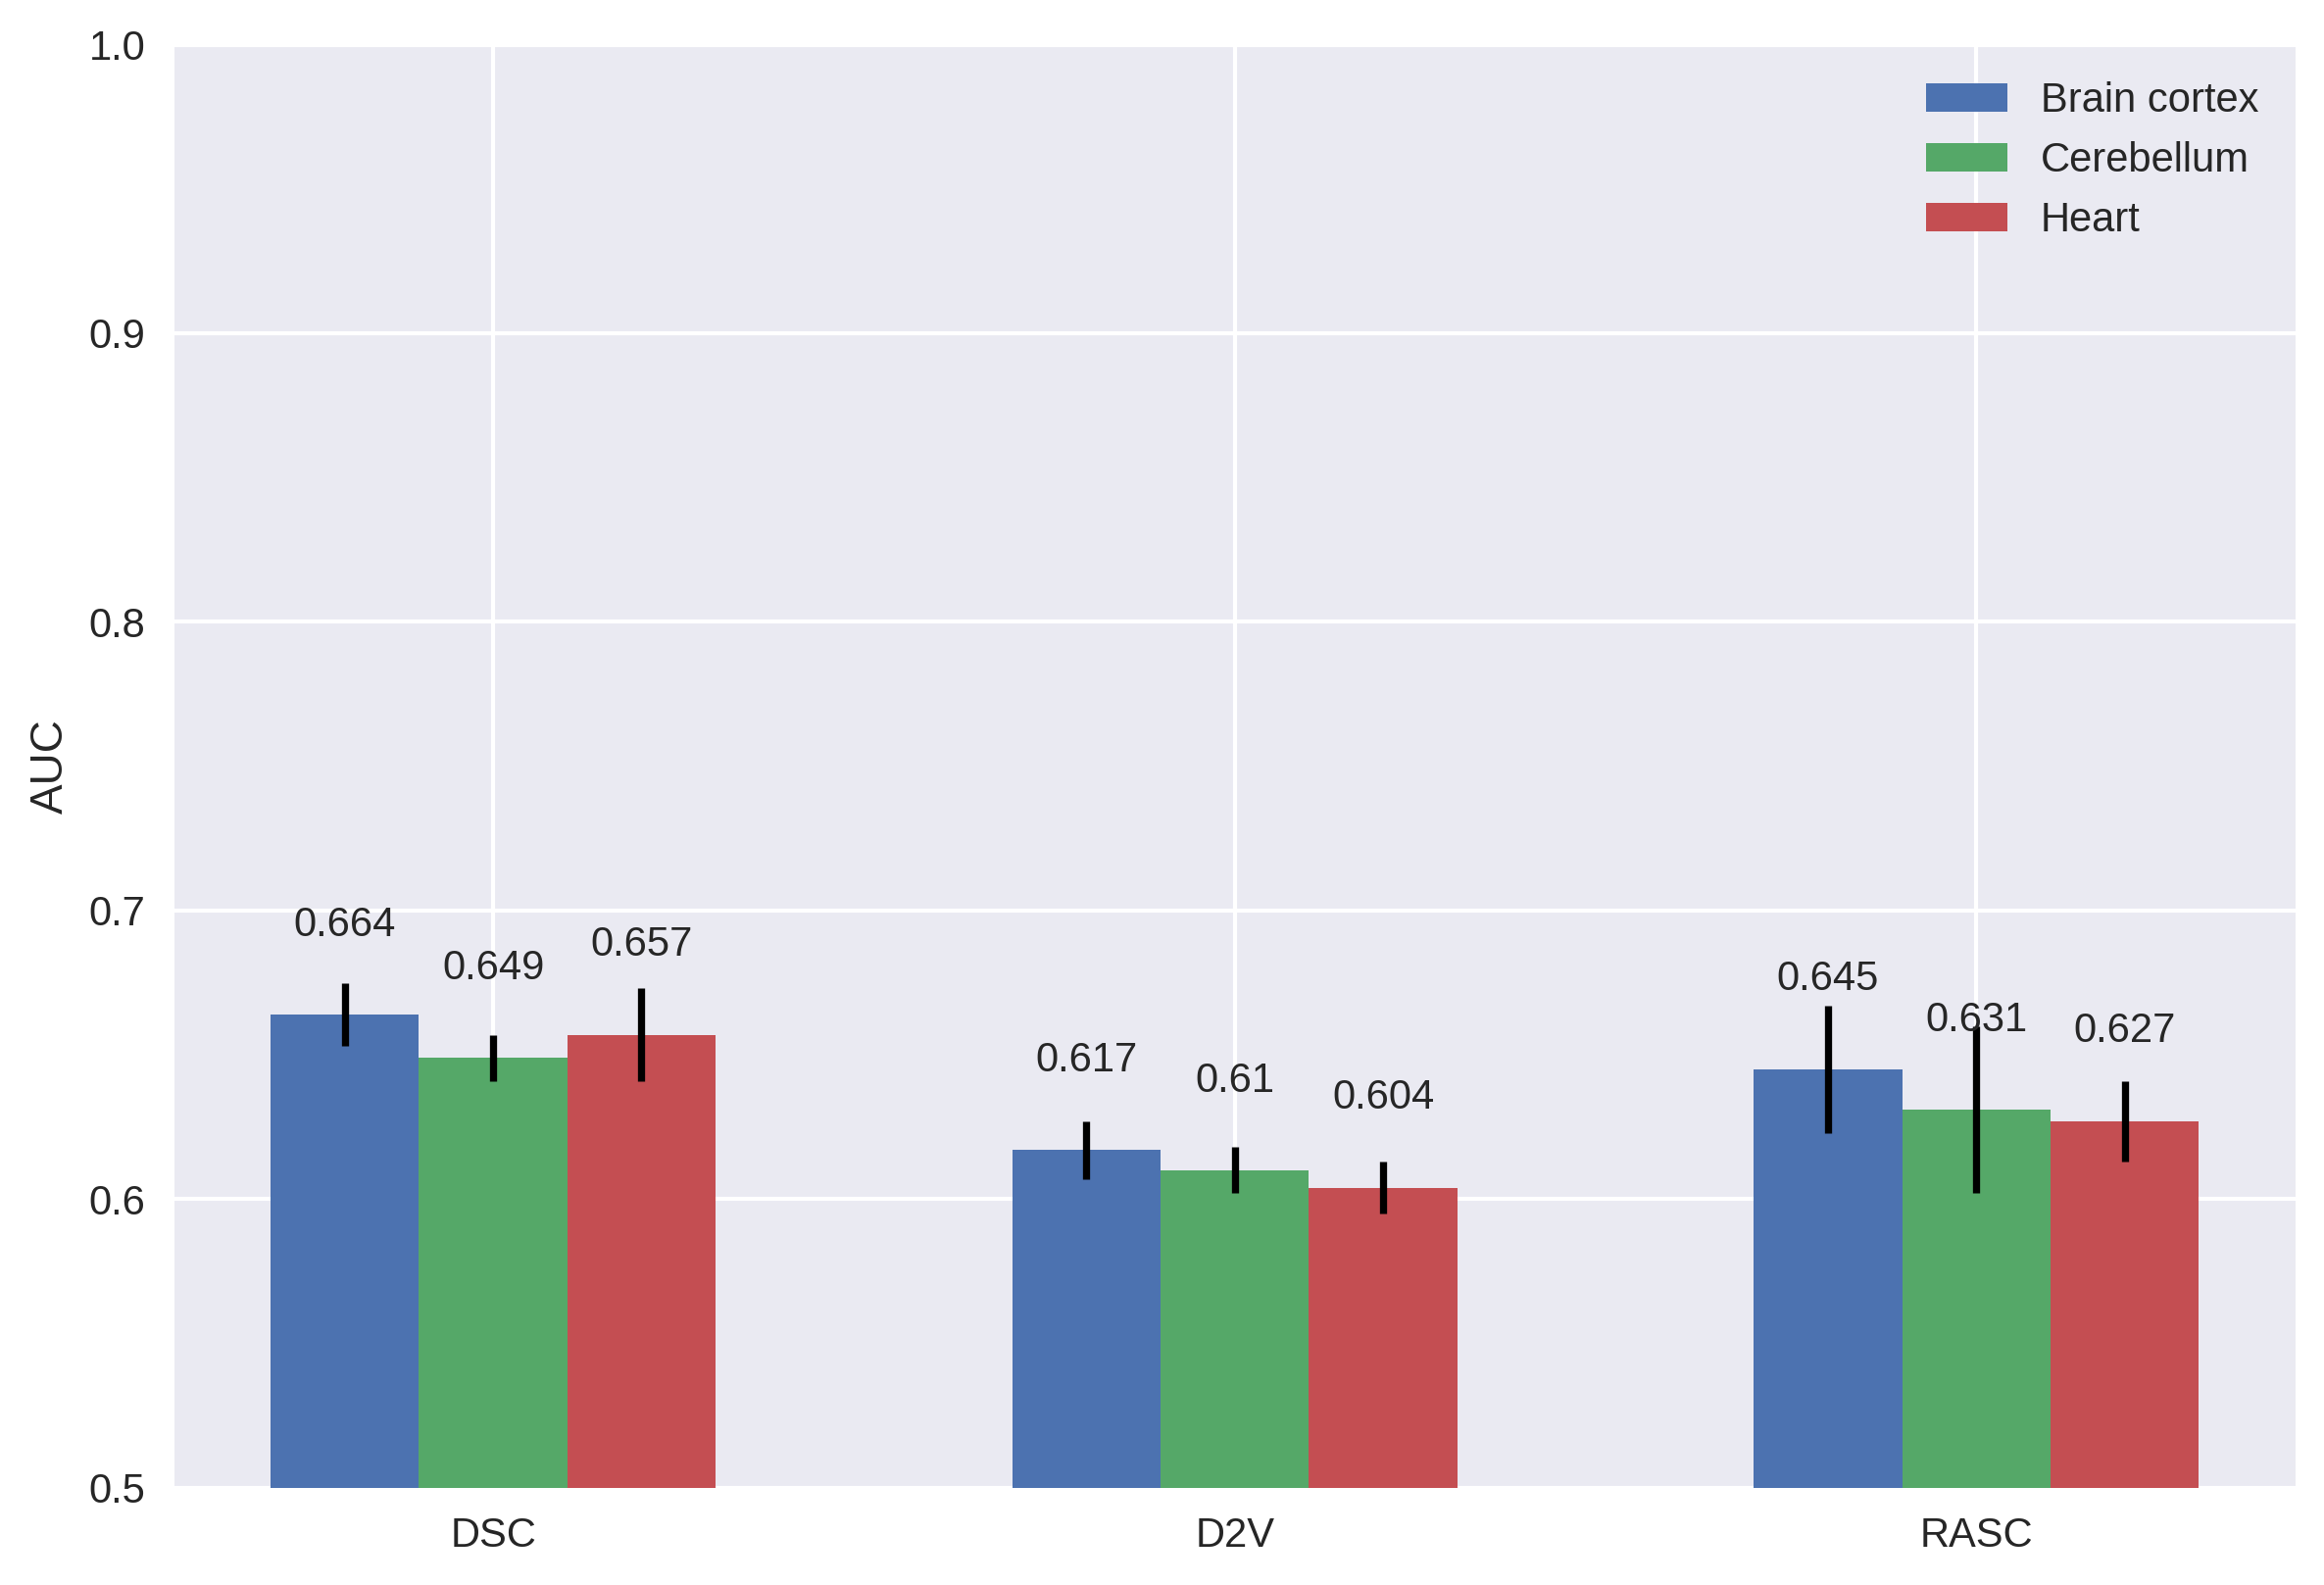
\includegraphics[width=0.85\textwidth]{../visualizations/ch5-results/gtex_exon_barcharts.png} 
	\caption{Performance on the GTEx-based exon-centric datasets across different tissues. The error bars give the standard deviation across all cross-validation runs. }
	\label{fig:gtex_exon_barcharts}
\end{figure}

\begin{figure}
%	\centering\includegraphics[width=0.7\textwidth]{../saved/log/GTEx_Exon_Brain_Attn/final/ROC.png} 
	\centering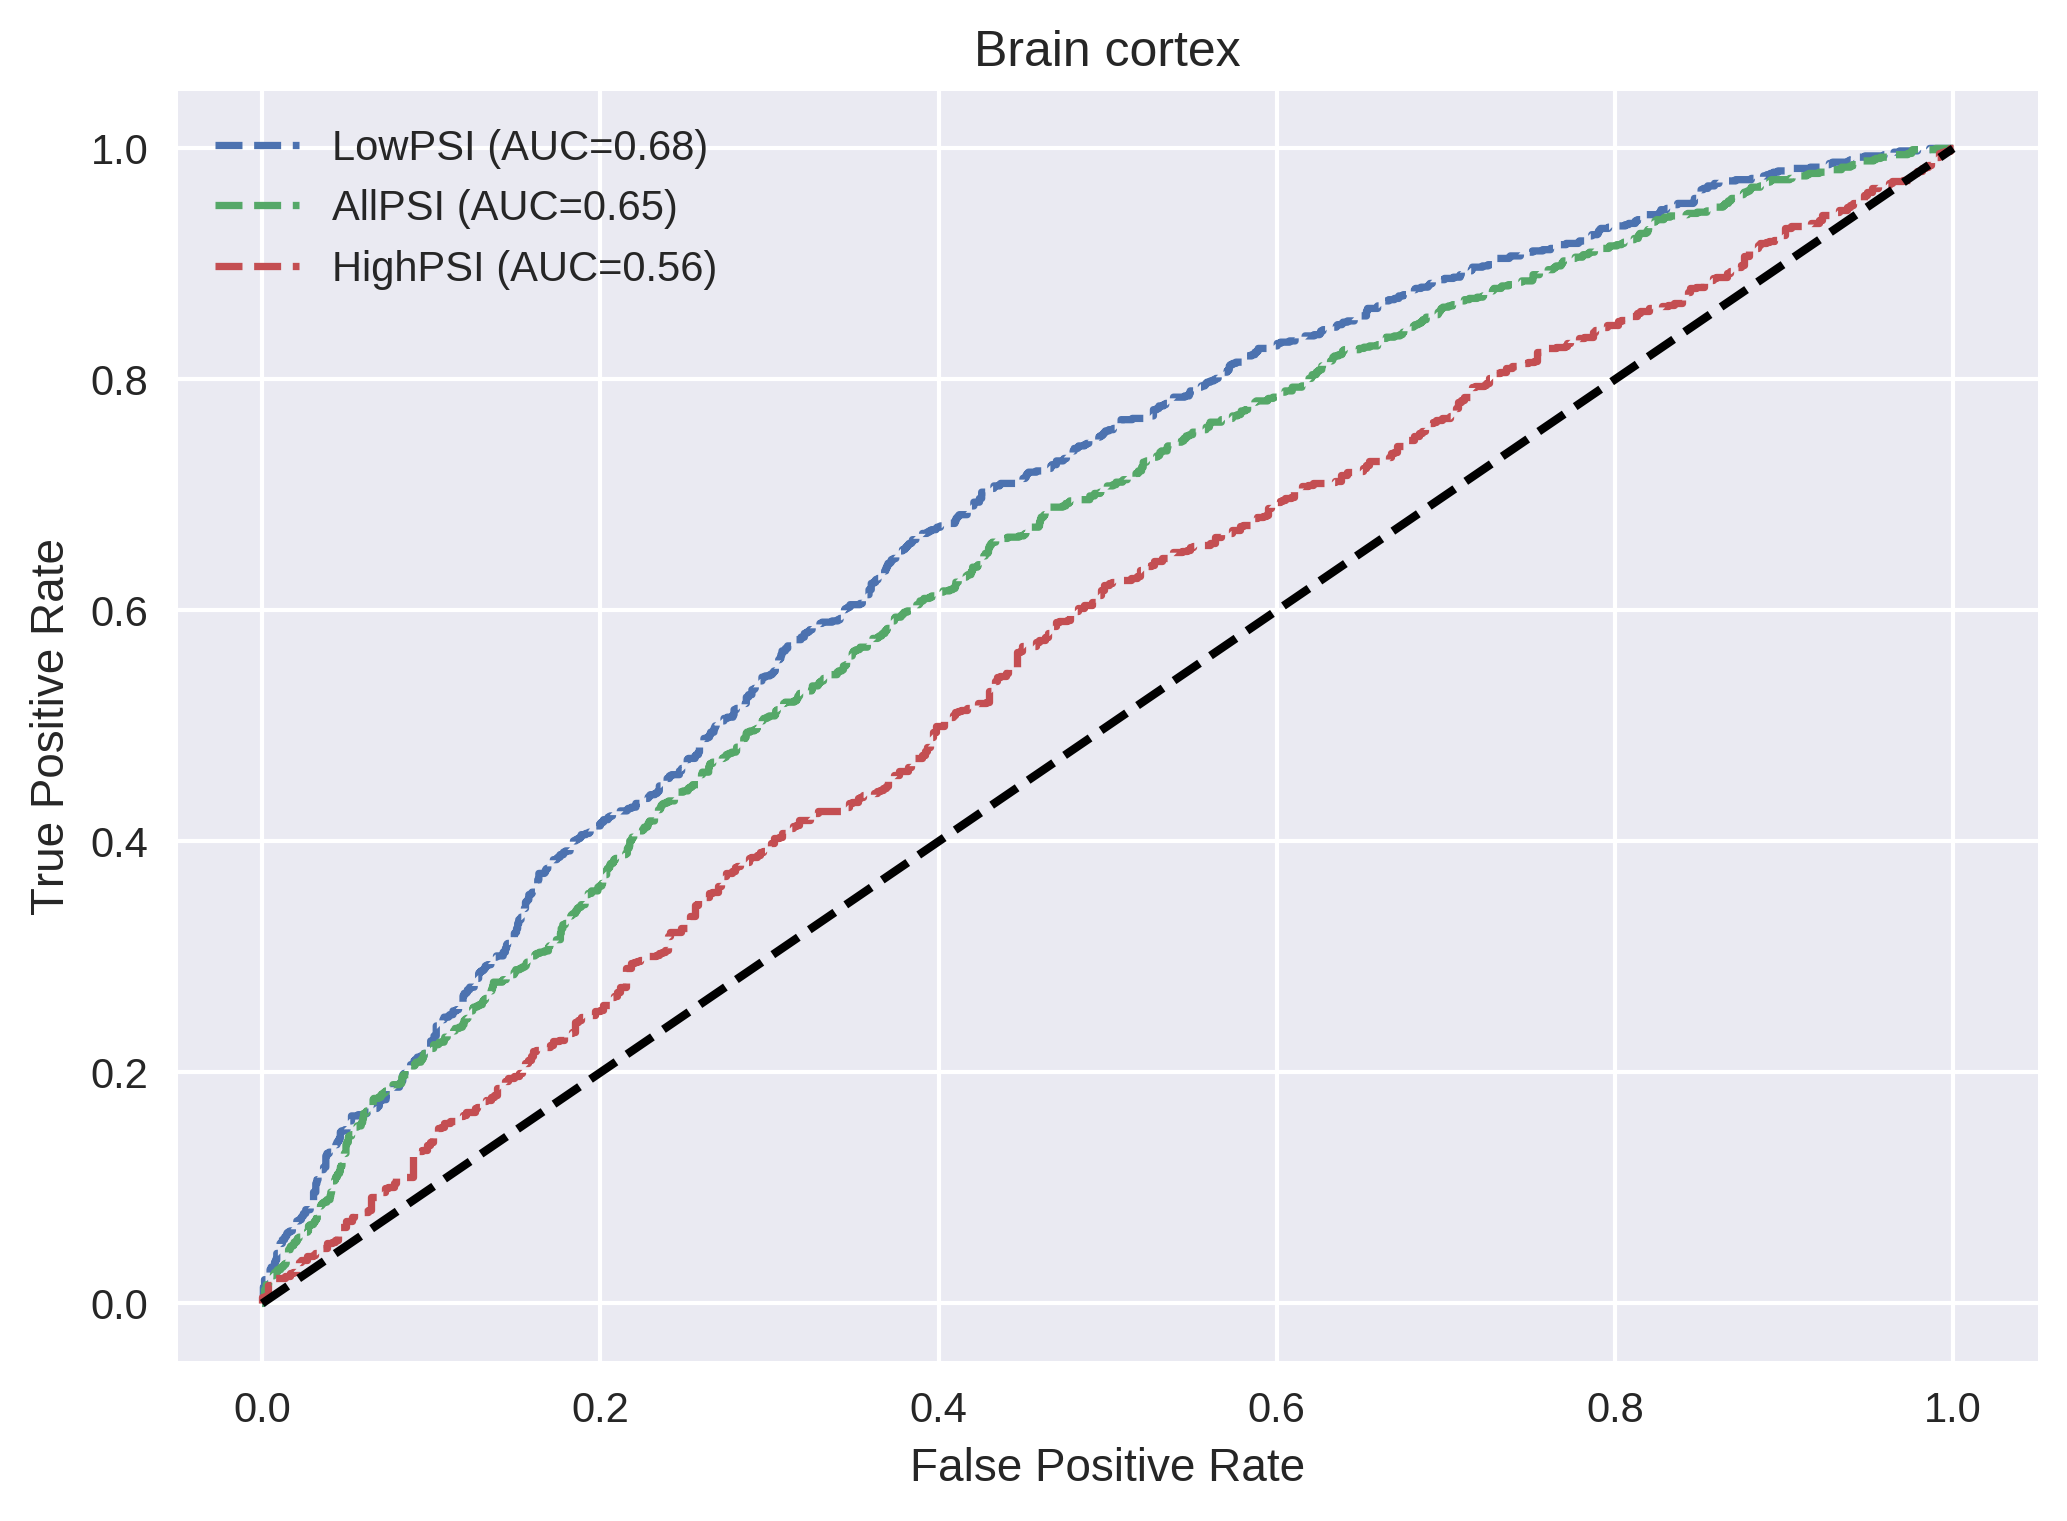
\includegraphics[width=0.7\textwidth]{../visualizations/ch5-results/gtex_exon_brain_roc.png} 
	\caption{
	ROC curve of RASC on GTEx-based exon-centric brain cortex dataset. 
  }
	\label{fig:gtex_exon_roc}
\end{figure}

Results are given in Figure \ref{fig:gtex_exon_barcharts}. Across all models, performance is poor and the predictive power of the models is low. Surprisingly, performance is also very similar across tissues: the mean cross-tissue performance difference of 0.007 AUC is smaller than the mean cross-run difference of 0.014 AUC. This is surprising from a biological perspective as cross-tissue splicing differences are well-documented \cite{crosstissuesplicing}. 
This could indicate that, while splicing across tissues varies, the relative complexity of cassette exon splicing behaviour across tissues is similar. However, this would be overinterpreting models with low predictive power.
Most likely, the models are already struggling to learn the baseline splicing behaviour invariant across tissues and don't learn finer cross-tissue differences. 
% that Since our models perform so poorly they likely already struggle to learn the baseline splicing behaviour invariant across tissues. 
The low cross-tissue performance differences also surprising from a machine learning perspective, as the cerebellum-based dataset contains almost twice as many training samples as the heart-based dataset. This indicates that either 1) the models have already hit a point of diminishing returns for adding more data or 2) the models generally require significantly more training samples. All models perform best on the dataset based on a brain cortex sample. %TODO: not happy with the wording of this section yet; could be more dense.
%even if splicing varies across tissues, performance as measured by AUC could be the same if roughly same level of complexity -- avoid this issue by referrering to it as most likely explanation

Relative model performance stays the same between tissues: DSC tends to perform best, followed by RASC and the D2V model. The variance of RASC between runs is on average twice as twice as high as the respective variance of DSC and D2V. As a result, RASC is the best performing model, as measured by the maximum rather than mean AUC value, on the brain cortex tissue-based and cerebellum tissue-based datasets. This indicates that RASC needed more regularization on this dataset and dataset specific fine-tuning could've lead to it performing the best across cross-validation runs.
%TODO: rerun RASC so it becomes the king again

Figure \ref{fig:gtex_exon_roc} gives more insight into model performance. 
%TODO: mention in methods section the dataset split
The performance on highly included, alternatively spliced exons (80\% <= PSI < 99\%) is significantly worse than on more rarely included, alternatively spliced exons (PSI < 80\%). Per AUC definition, the AUC on the allPSI dataset lies in-between these two extremes. In this case, only ~28\% of alternatively spliced exons belong to the exons with a high PSI and therefore the combined AUC is heavily weighted towards the AUC on the exons with low PSI. These observations mirror analogue observations made on the HEXEvent dataset \cite{dsc}.

%---- removing length feature would be interesting; doing it on brain as best performance and sort of lowest combined variance\\


%- could note that in earlier variation of the dataset where no TPM treshold was used (?) the networks didn't learn anything\\
%	-- would be great finding out / remembering what exact step is the crucial one
%	




%\textbf{conclusions:}\\
%	- performance generally poor\\
%	- inter-tissue variance low\\
%	- due to issues with GTEx data, likely desirable to test with other datasets
	
	
	

\subsection{Intron-centric datasets} \label{subsec:gtex_junc}

\begin{figure}[h]
	\centering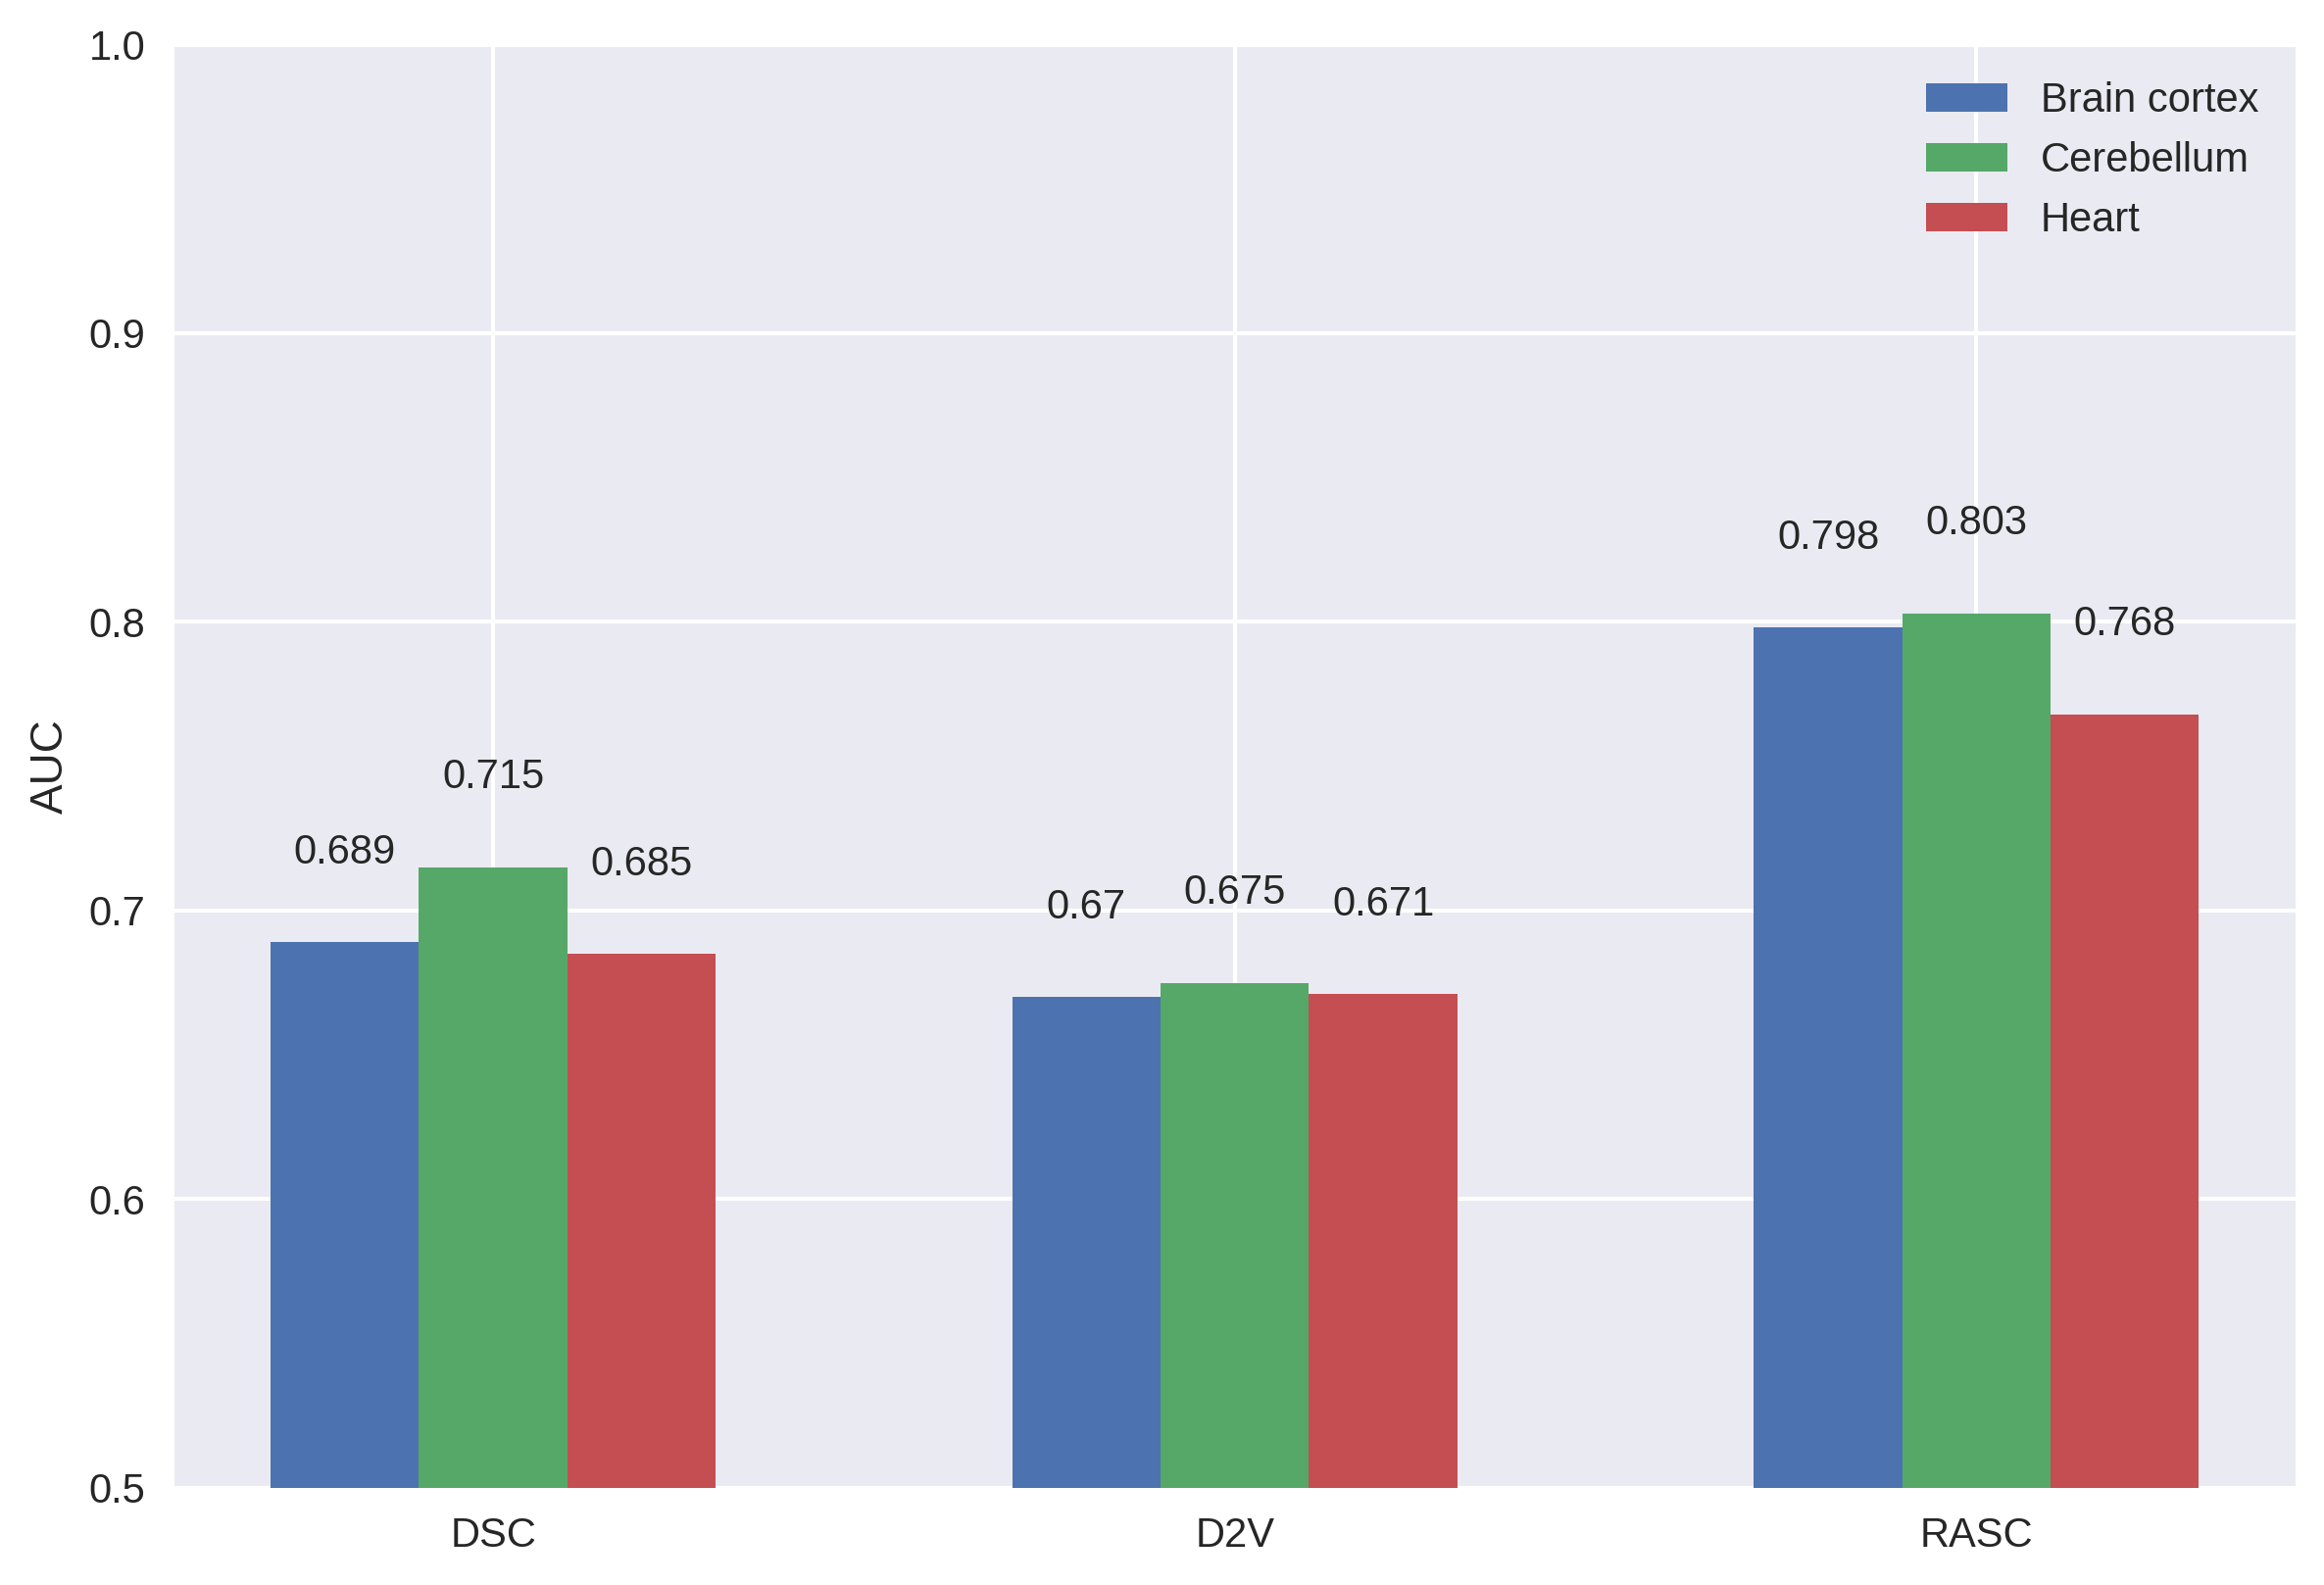
\includegraphics[width=1\textwidth]{../visualizations/ch5-results/gtex_junc_barcharts.png} 
	\caption{Performance on the GTEx-based junction datasets across different tissues. }
	\label{fig:gtex_junc_barcharts}
%	TODO: should these bars move closer together?
\end{figure}


\begin{figure}[h]
%	\includegraphics[width=0.5\textwidth]{../saved/log/GTEx_Junc_Heart_DSC/final/ROC.png} 
%	\includegraphics[width=0.7\textwidth]{../saved/log/GTEx_Junc_Heart_Attn/junc_cv_final/ROC.png}
	\centering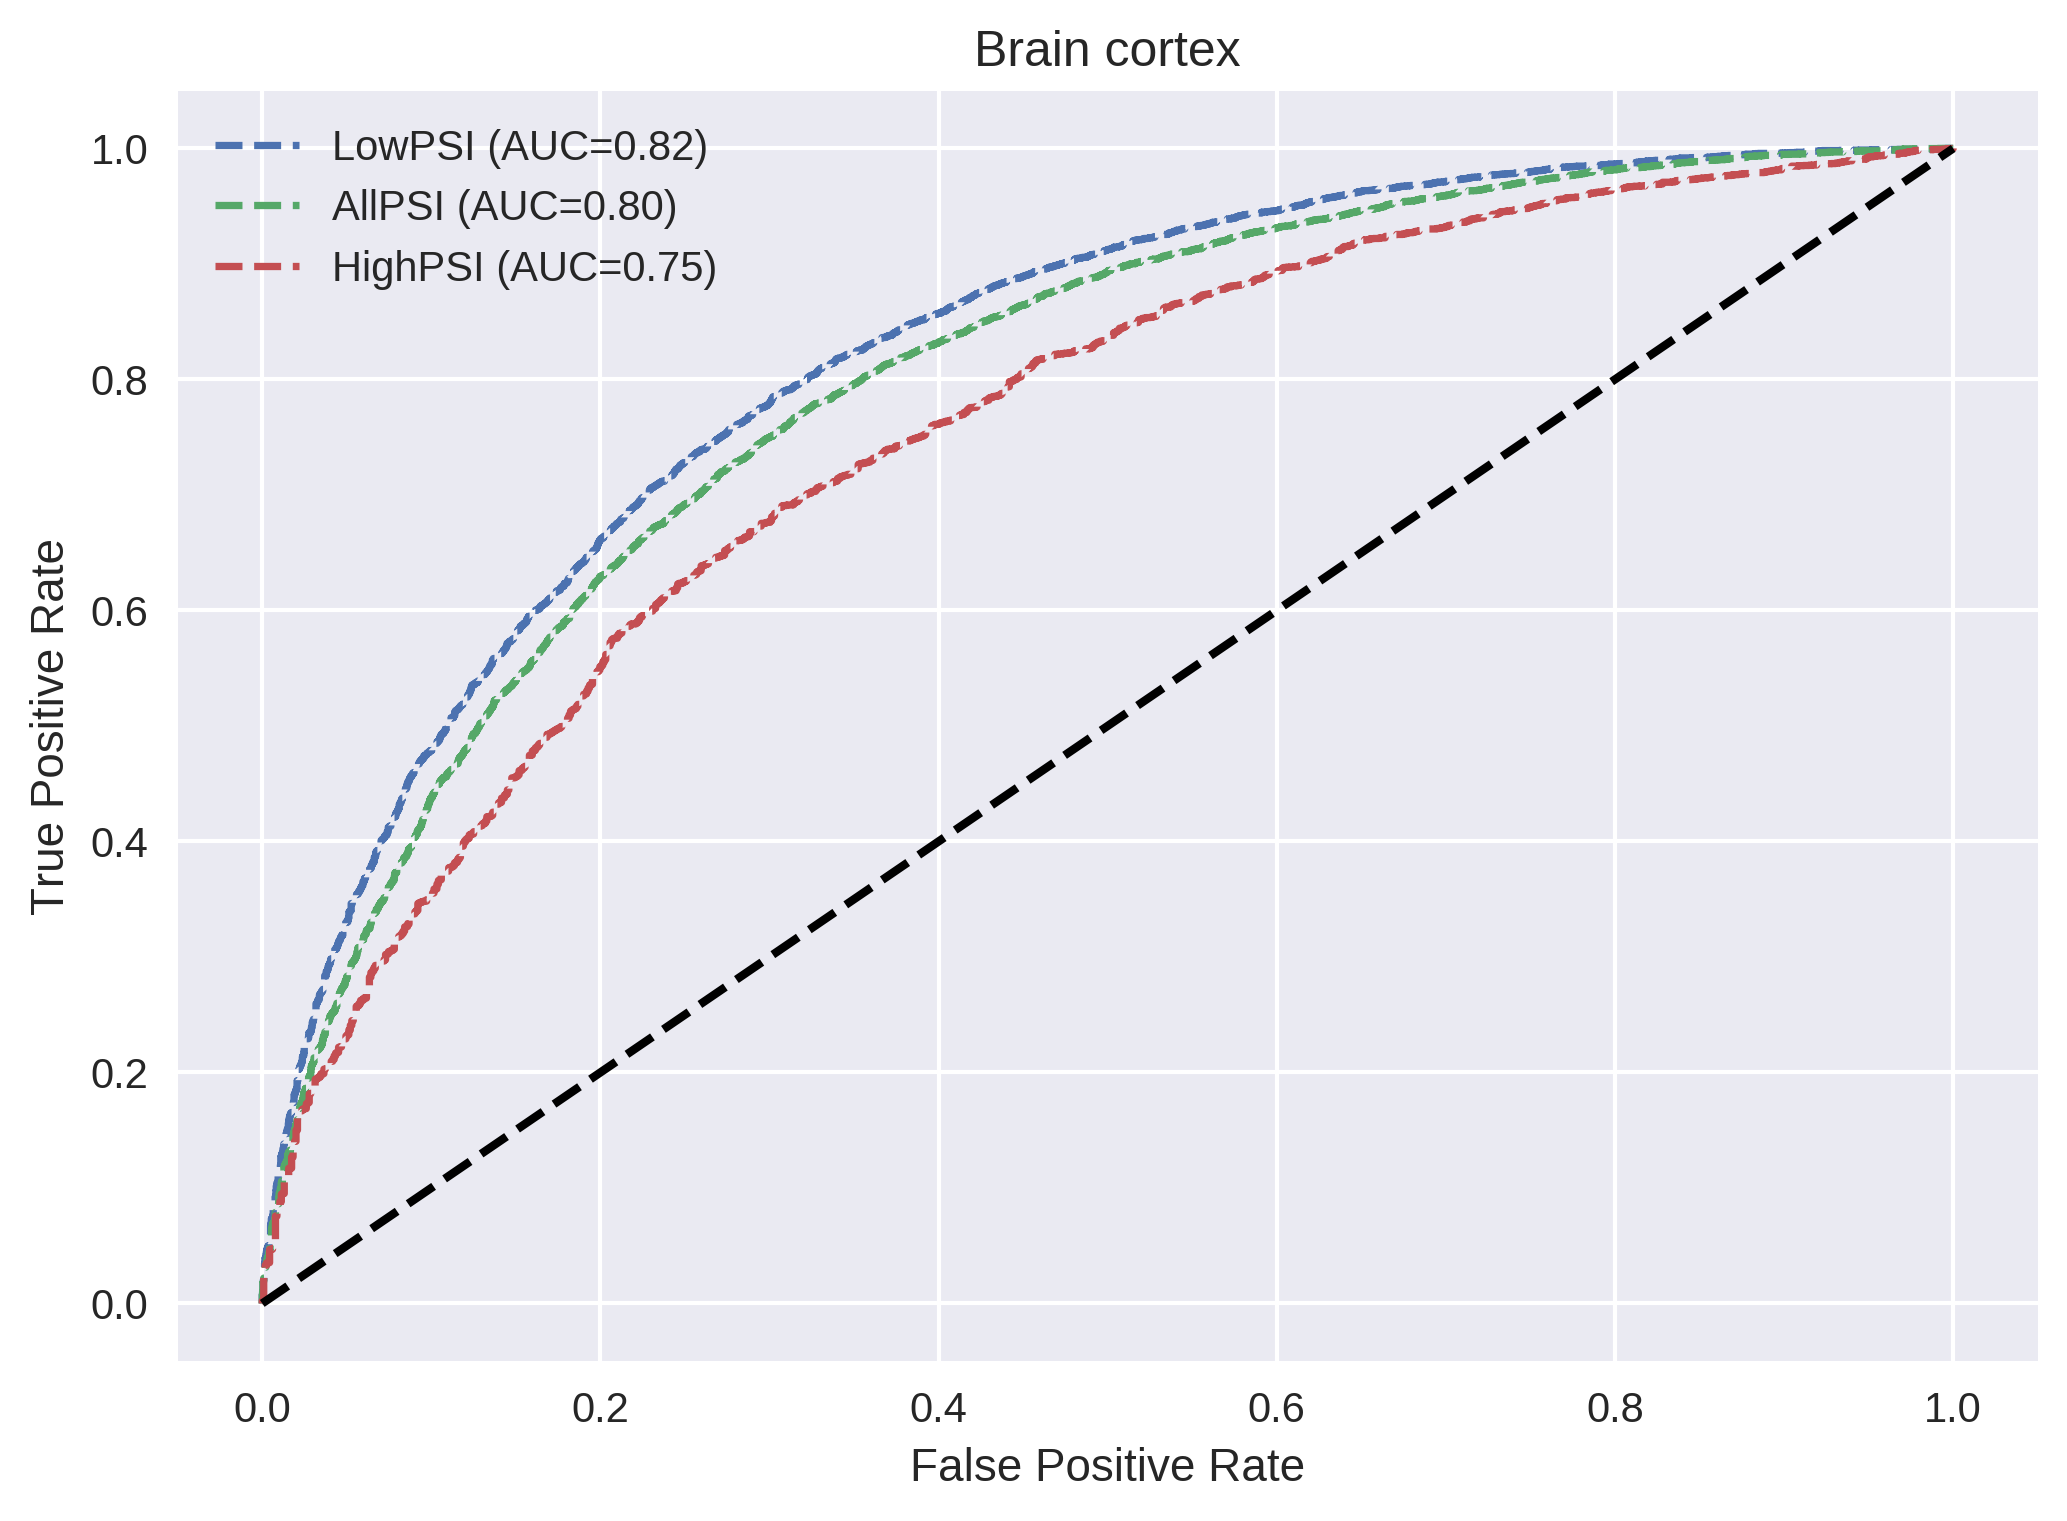
\includegraphics[width=0.7\textwidth]{../visualizations/ch5-results/gtex_junc_brain_roc.png} 
	\caption{ROC curve from training RASC on the GTEx-based intron-centric heart-tissue-based dataset. }
	\label{fig:gtex_junc_rocs}
\end{figure}


%TODO: motivation for using junction-centric datasets
\subsubsection{Main analysis}
Figure \ref{fig:gtex_junc_barcharts} shows that junction classification is seemingly an easier task: the AUC of all models increases by at least 0.05 to 0.06 compared to the exon classification task. However, this is likely a result of the intron-centric datasets containing on average four times more training samples rather than due to different inherent task difficulties. RASC significantly outperforms DSC and D2V. 

Similar to the exon-centric datasets \ref{subsec:gtex_exon}, we observe very low cross-tissue performance differences. We again believe that model performance is generally too poor to warrant speculation about the underlying biological realities. However, we come to a different conclusion regarding the observation that the different dataset sizes between tissues don't affect model performance:
for the GTEx-based exon-centric datasets we hypothesized that the models have hit diminishing returns for adding more data or that they need significantly more data. As the number of training samples has quadrupled in the move from exon- to intron-centric datasets, we now believe that the models have hit a point of diminishing returns for adding more data. 


%TODO: rerun heart tissue experiments with proper 0.4 dropout so that fucking variance disappears


The performance across rarely and highly included junctions is less disparate than on the exon-centric datasets (see Figure \ref{fig:gtex_junc_rocs}). This indicates that the models are better able to learn to recognize motifs which separate constitutive and highly alternatively spliced junctions than for exons.
%However, this observation may not be very epistemiologically certain as only 15\%
%TODO explanation for this

\subsubsection{Assessing model performance without length features}

\begin{table}[h!]
	\centering
	\begin{tabular}{| l | c | c | c| c} 
		\hline
		Model name & Only sequences & Sequences + lengths & Relative performance improvement\\
		\hline
		DSC & 0.661 & 0.704 & 0.211\\
		D2V & 0.629 & 0.673 & 0.254\\
		RASC & \textbf{0.776} & \textbf{0.808} & 0.104\\
		\hline
	\end{tabular}
	\caption{Performance on the GTEx-based intron-centric dataset with and without length features. 
		%		Note that the relative performance drop was computed with reference to the baseline AUC value of 0.5.
	}
	\label{table:gtex_junc_nolens}
\end{table}
%TODO: overlaps to the right side
As model performance is more promising than on the GTEx-based exon-centric datasets, we validate that this isn't due to an overreliance on the length features as on the HEXEvent dataset. Table \ref{table:gtex_junc_nolens} shows that the length features still make up a large part of model performance, but that the models don't rely on them completely. However, the performance proportion the length features account for is still biologically implausible. %TODO: citation needed?
Thus we conclude that the dataset is an improvement over the HEXEvent dataset, but generating a dataset where model performance is less dependent on the length features is still desirable. 


%15 \% of alternatively spliced exons are highly included 

%\subsection{Reconstructing HEXEvent-dataset with GTEx data}
%- dataset where I only took exons which were also in GTEx data\\
%- seriously considering not showing these results as I basically already debunked HEXEvent at this point -- so from a narrative perspective, why spend effort on replicating it?

\subsubsection{Evaluation of the GTEx-based datasets}
Overall, we observe poor to promising model performance, biologically surprising low cross-tissue performance differences and biologically implausible reliance on the length features. 
In \ref{subsubsec:naivepsi}, we mentioned issues when trying to estimate PSI naively. Although we alleviated these in pre-processing, we don't account for the information contained in non-junction reads and don't integrate information from multiple samples. As a result, data quality is likely still an issue distorting the results in this section. 
Thus we conclude that the GTEx-based datasets improve upon the HEXEvent dataset, but using datasets based on more accurate PSI estimation methods is desirable and would lead to more meaningful results. %would lead to more meaningful results.

%Alleviating these issues, we next evaluate the models based on a primary data source which gives access to raw RNA-seq reads. This enables us to use methods from the literature which leverage information from non-junction reads and multiple samples.

%Overall, we observe poor model performance and biologically surprising low cross-tissue performance differences. This indicates that the GTEx-based exon-centric dataset is not fit for training neural-network based splicing codes and conclude that evaluating the models on other datasets is desirable.



\section{HipSci SUPPA datasets} \label{subsec:hipsci_suppa}
\subsection{Dataset based on sensory neuron cell lines}

\begin{figure}
	\centering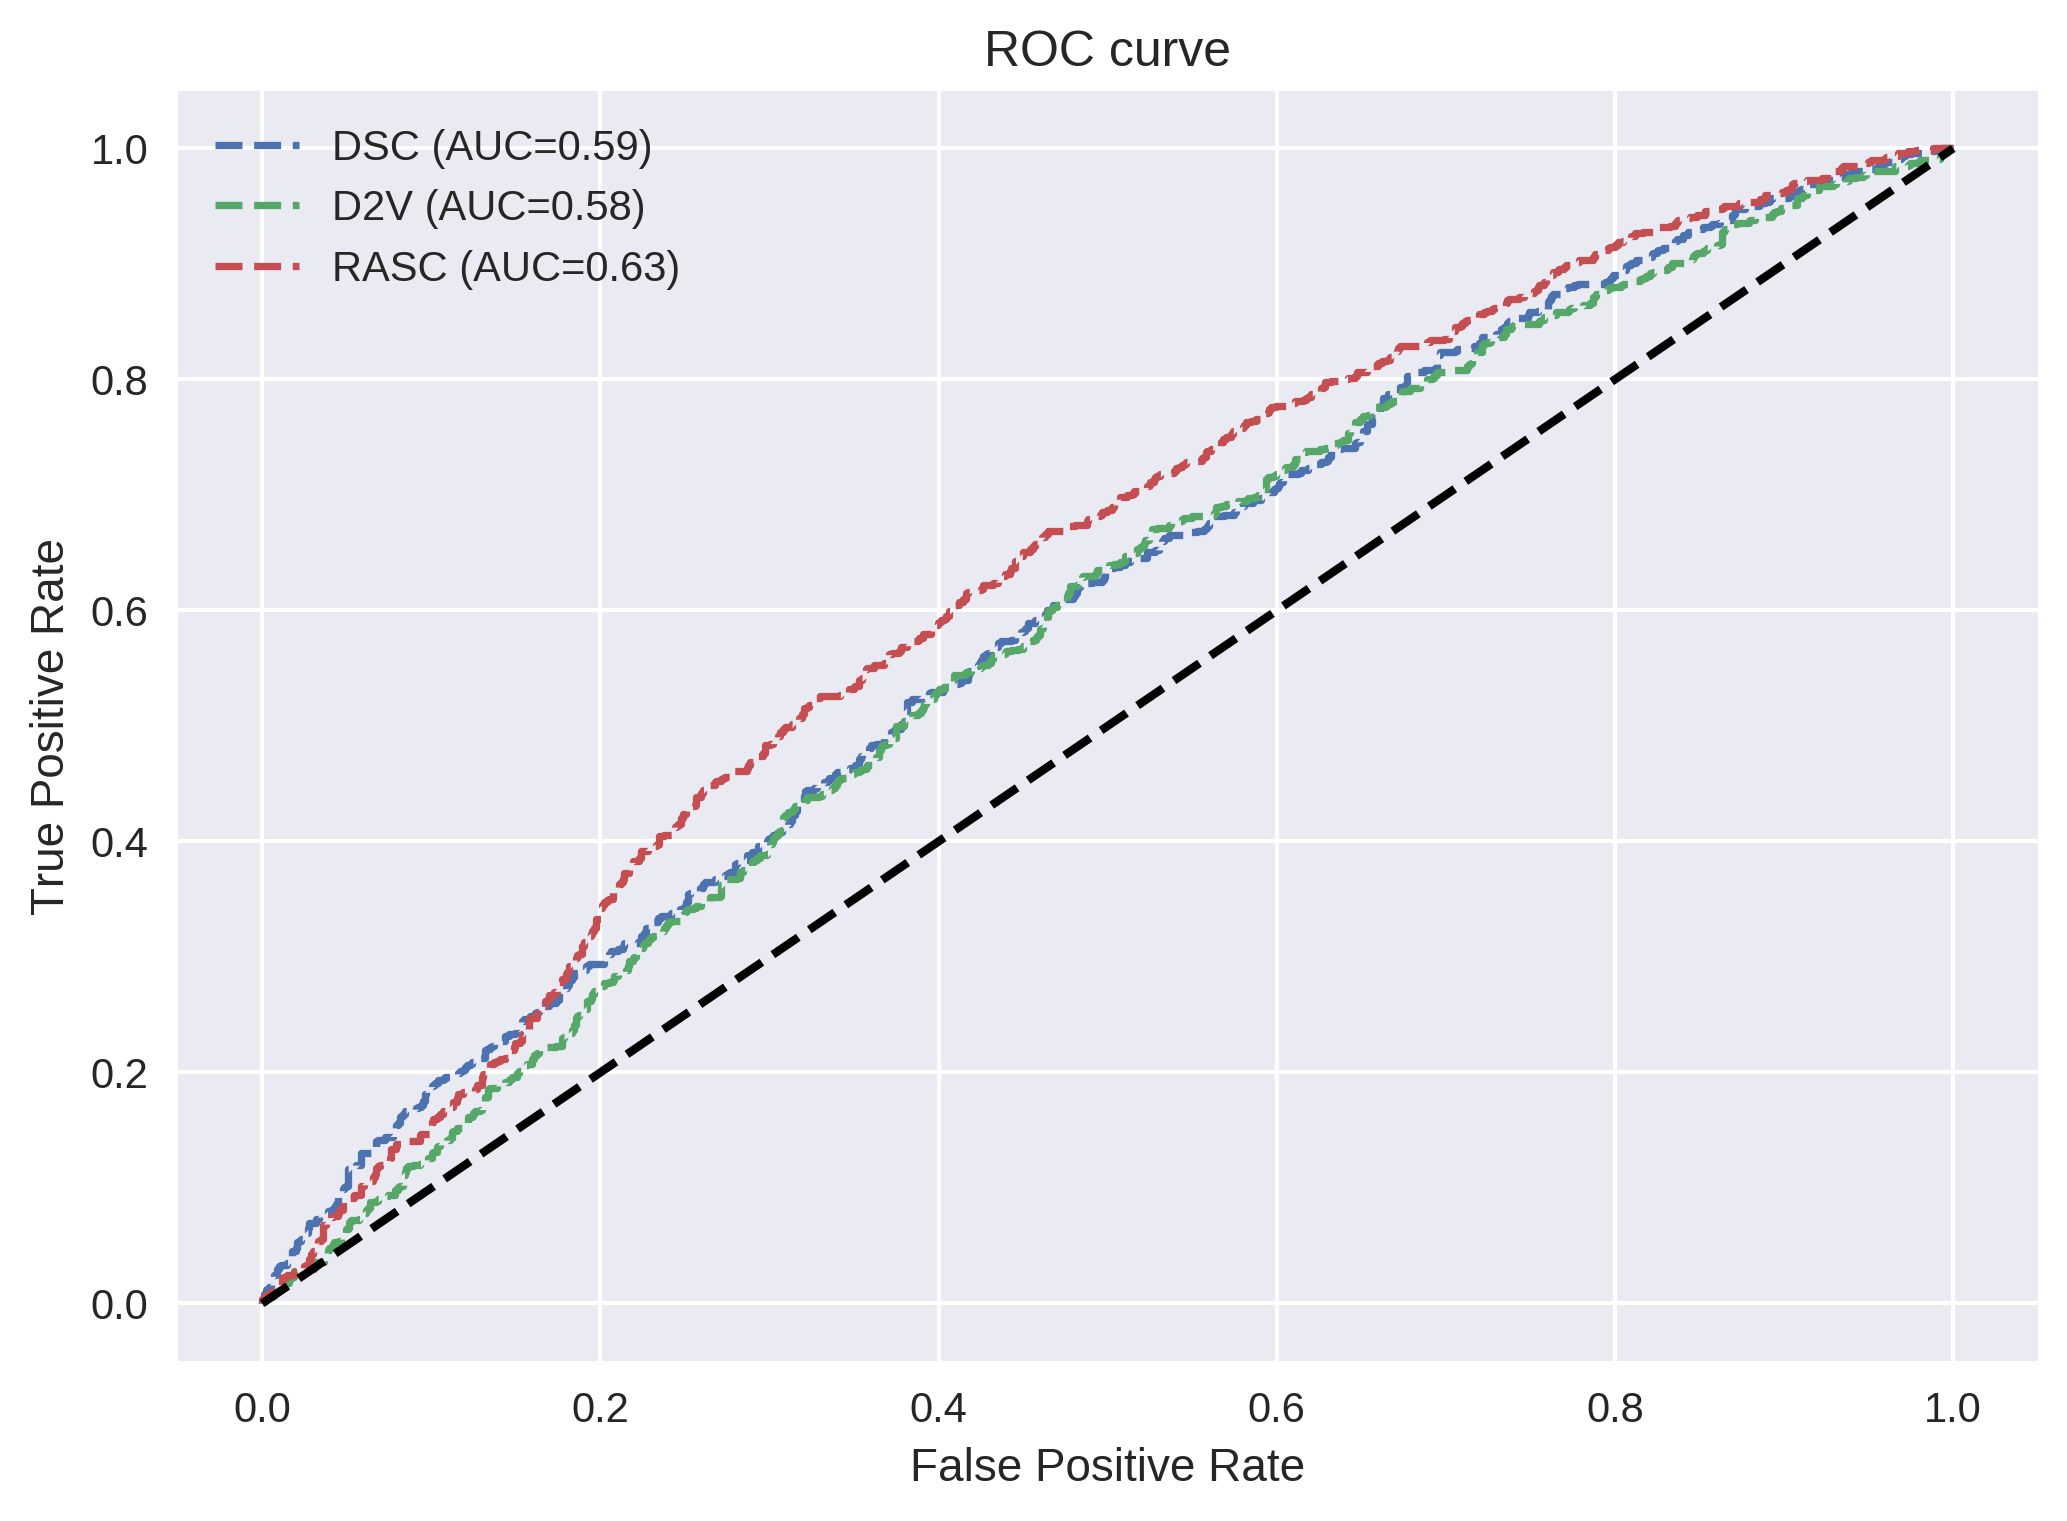
\includegraphics[width=0.7\textwidth]{../visualizations/ch5-results/suppa_cross_model_roc_auc_comparison.png} 
	\caption{Comparison of the ROC curves of the three models on the HipSci SUPPA dataset. The dataset is based on iPSC cell lines differentiated to sensory neuron cell lines. }
	\label{fig:suppa_auc_roc}
\end{figure}
\subsubsection{Main analysis}
Figure \ref{fig:suppa_auc_roc} shows how the model perform very poorly on the HipSci SUPPA dataset. The performance is worse than on the GTEx-based exon-centric dataset and roughly equal to the performance on the HEXEvent dataset without length features. This indicates that 
\begin{enumerate}
	\item either we arrive at a strong dataset here and that constitutive exon classification is more challenging than so far anticipated,
	\item or this dataset suffers from data quality issues which make constitutive exon classification very challenging for the models.
\end{enumerate}

Among these two, 2. is more likely due to SUPPA not addressing various challenges in PSI estimation and due to SUPPA not generating constitutive training samples (see also \ref{subsubsec:suppa}). SUPPA does not appear to be accurate enough for our purposes. Therefore, we don't evaluate our models on the HipSci SUPPA dataset based on undifferentiated iPSC cell lines.


%in retrorespect, SUPPA was not the best choice for dataset processing. It operates at a transcript level and therefore implicitly relies on the assumption that all transcripts of a given gene are known - this is often not the case. Additionally, it does not make it possible to generate a list of non-cassette constitutive exons, therefore roughly halving the size of the training set and the number of samples the model can learn from. Its PSI estimation is very simplistic and doesn't account for multiple of the issues highlighted in \ref{subsec:psiestimation}. Thus, we now turn to data processing with MAJIQ in hopes of better results. 

% TODO thought: what if AUC here is only worse because the model doesn't have easy to classify constitutive exons which boost the AUC? 


\section{HipSci MAJIQ datasets} \label{subsec:majiq}

\subsection{Dataset based on sensory neuron and iPSC cell lines}\label{sec:hipsci_neuron_majiq}

%\begin{figure}
%	\centering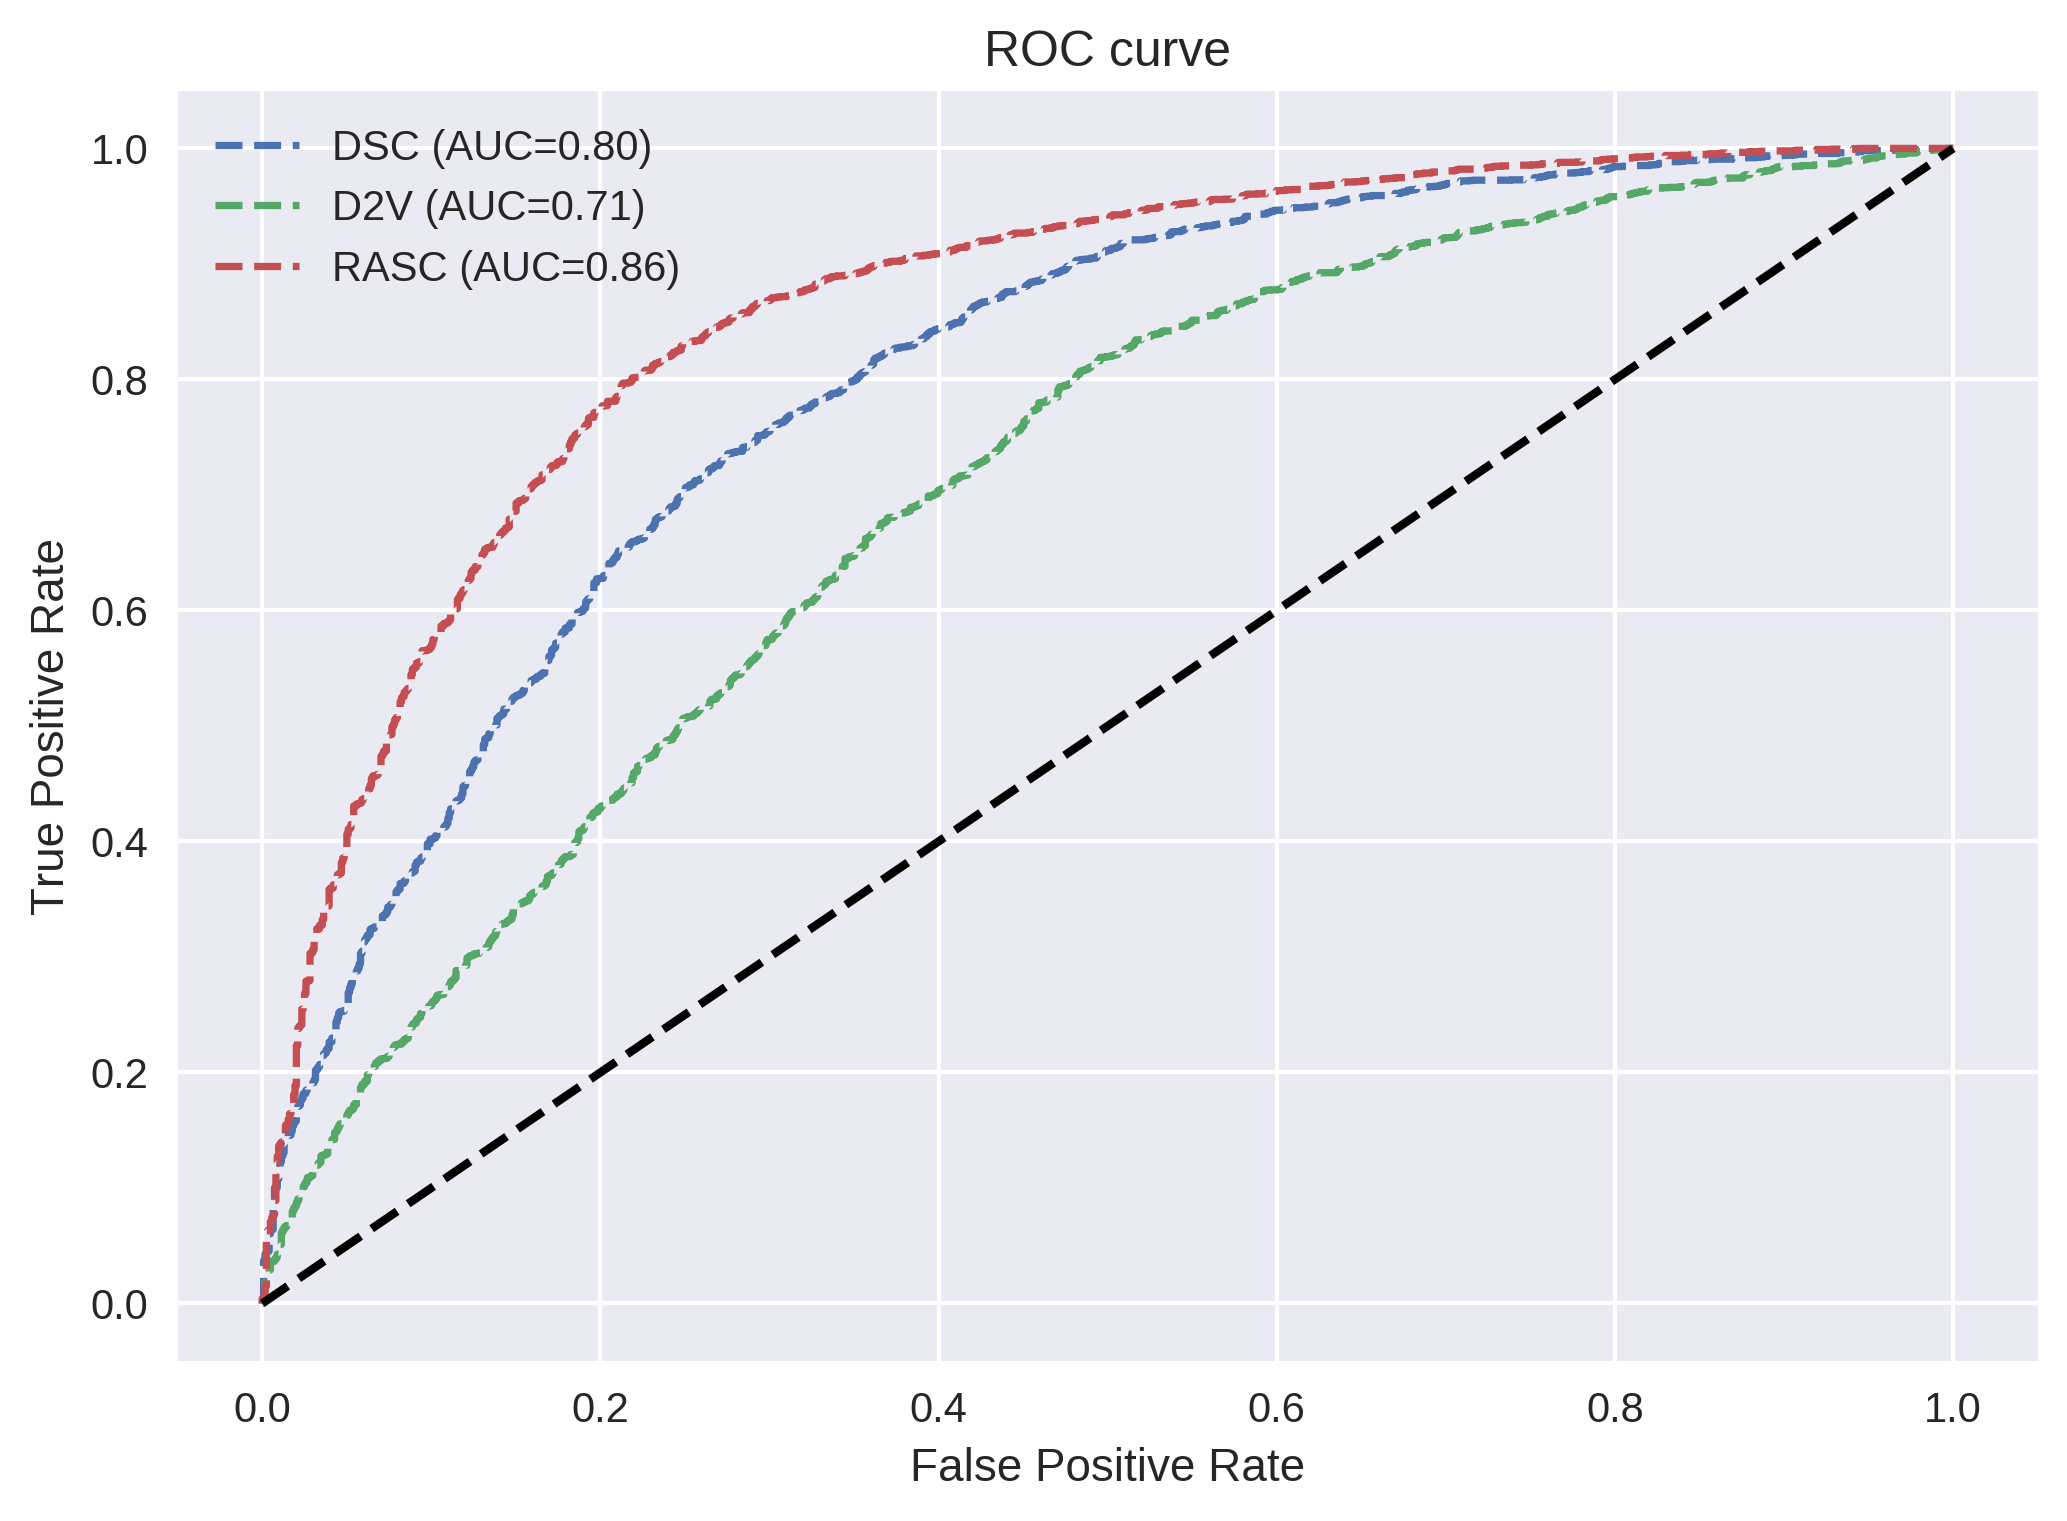
\includegraphics[width=0.49\textwidth]{../visualizations/ch5-results/majiq_neuron_cross_model_roc_auc_comparison.png} 
%	\centering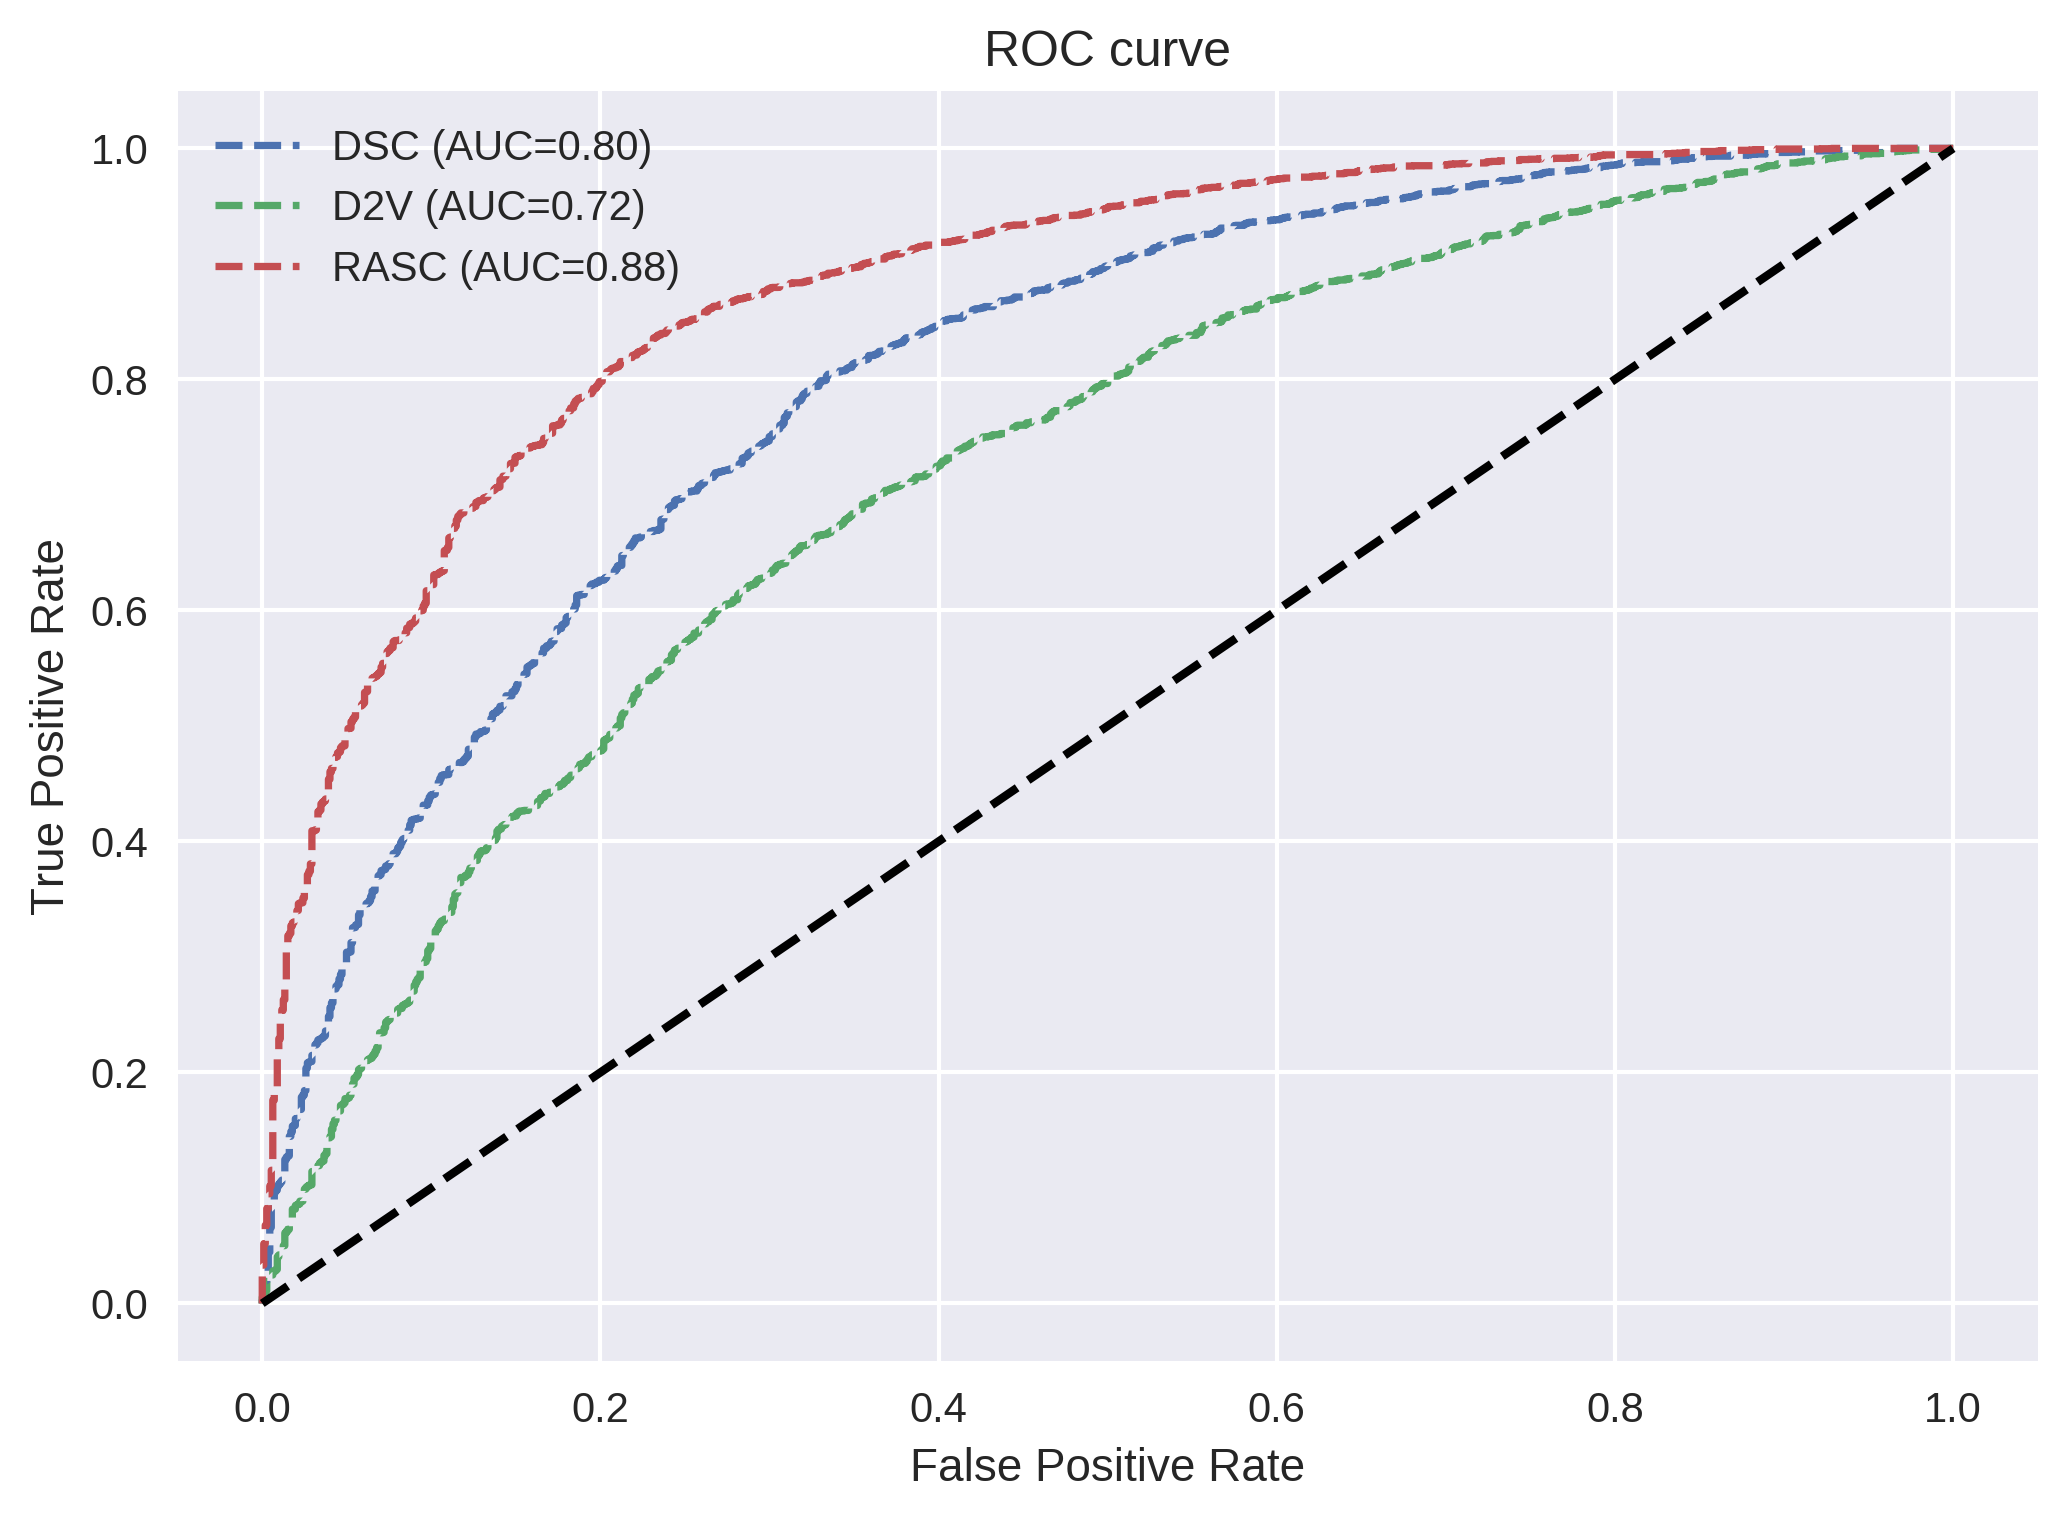
\includegraphics[width=0.5\textwidth]{../visualizations/ch5-results/majiq_ipsc_cross_model_roc_auc_comparison.png} 
%	\caption{Left: ROC curves on dataset based on processing with MAJIQ and iPSC cells differentiated to neurons. Right: ROC curves on dataset based on processing with MAJIQ and undifferentiated iPSC cells. }
%	\label{fig:majiq_rocs}
%\end{figure}


%TODO: replot after iPSC runs redone
\begin{figure}
	\centering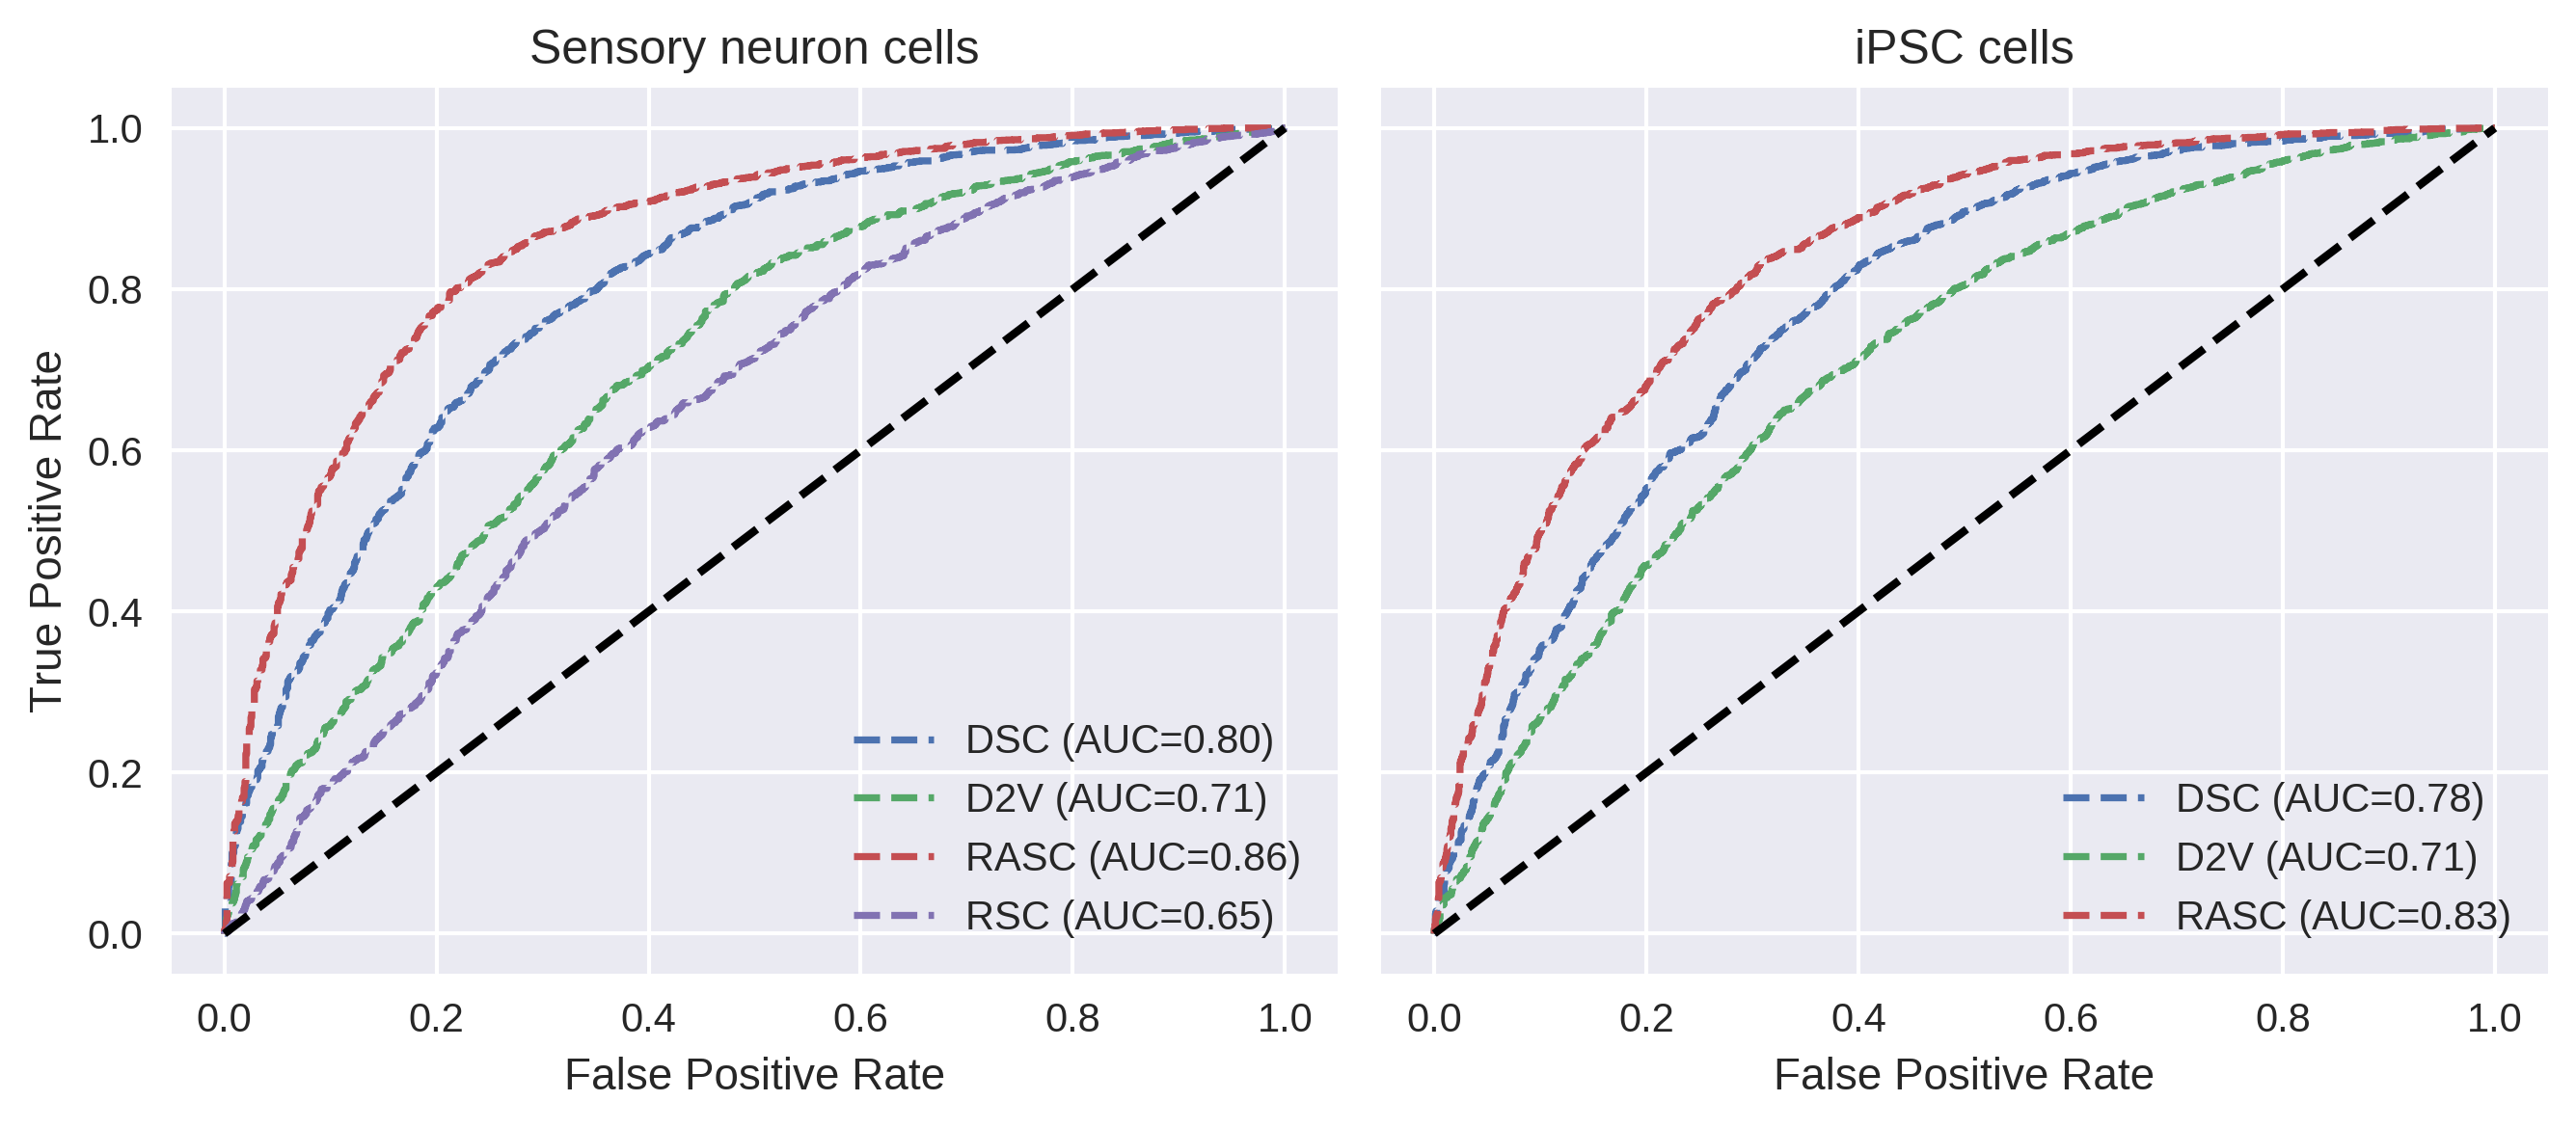
\includegraphics[width=1\textwidth]{../visualizations/ch5-results/majiq_neuron_ipsc_cross_model_roc_auc_comparison.png} 
	\caption{Left: ROC curves on HipSCi MAJIQ dataset derived from iPSC cells differentiated to neurons. Right: ROC curves on HipSCi MAJIQ dataset derived from undifferentiated iPSC cells. }
	\label{fig:majiq_rocs}
\end{figure}

\subsubsection{Main analysis}
All models perform significantly better than on previous datasets and we observe stark disparities between the models (see Figure \ref{fig:majiq_rocs}). While DSC outperforms D2V by a significant margin, it is outperformed by a similar margin by RASC. Adding attention to RSC promotes it from the worst to the best performing model, validating our choice. 

%The dataset based on undifferentiated iPSC cells seems to be less challenging: the AUCs are roughly 0.02 higher than on the dataset based on sensory neuron cells. At a closer look at the dataset distribution....

% TODO: investigate whether this is just a result of dataset composition --> not at first look
% neuron: 26394 / 8201 / 10151 = 44746
% ipsc: 27371 / 9299 / 11819 = 48489
% --> look at relative numbers, once you have analyzed across tissue-performance

% TODO: change roc curves such that I give AUC values explicitly (better than alternative of redoing)

%todo thought: it would be interesting to reevaluate all models without constitutive exons to see whether they actually perform better than in suppa dataset

\subsubsection{Impact of architectural choices} \label{subsubsec:majiq_architectural_choices}
The poor performance of D2V is likely a result of its architecture: the 100-dimensional embeddings used for classification weren't optimizely jointly during training and likely don't contain fine-grained information, such as the specific positons of motifs, required for accurate splicing prediction. We conjecture that D2V would benefit from receiving further split input sequences, e.g. input sequences containing 35 nucleotides. The best solution, while keeping the word embeddings, would likely be to embed the overlapping 3-mers in the sequence via word2vec and combine this with an efficient convolutional architecture, as done in \cite{d2vsplicing}.



\subsubsection{Assessing the dataset quality}

\begin{table}[h!]
	\centering
	\begin{tabular}{| l | c | c | c| c} 
		\hline
		Model name & Only sequences & Sequences + lengths & Relative performance improvement\\
		\hline
		DSC & 0.811 & 0.808 & -0.010\\
		D2V & 0.665 & 0.715 & 0.233\\
		RASC & \textbf{0.853} & \textbf{0.865} & 0.033\\
		\hline
	\end{tabular}
	\caption{Performance on the dataset based on processing with MAJIQ and iPSC cells differentiated to neurons with and without length features given. 
		%		Note that the relative performance drop was computed with reference to the baseline AUC value of 0.5.
	}
	\label{table:majiq_nolens}
\end{table}
%TODO: overlaps again
As litmus test for dataset quality, we repeat the experiment of removing the length features as model input. We document the results in Table \ref{table:majiq_nolens}.
They reveal that a large part of D2V's performance relies on information contained in the length features. However, since removing the length features only marginally affects the performance of DSC and RASC, we conclude that the dataset is not biased in the same way as the HEXEvent dataset and that this observation is symptomatic of D2V being unable to effectively incorporate information from the sequences (see discussion in \ref{subsubsec:majiq_architectural_choices}). 

Giving the strong model performance independent of the length features and the prior expectation for MAJIQ to produce the highest quality PSI estimates, we conclude that it does. This indicates that the comparatively poor performance on the GTEx-based and HipSci SUPPA datasets are due to poor data quality, and not due to the inherent difficulty of the splicing classification task. Thus, using the HipSci MAJIQ datasets is preferable to using any of the other datasets we have evaluated. 

Motivated by this observation, we use the HipSci MAJIQ dataset to validate our architectural choices for RASC and to carry out further analysis omitted on the other datasets.





\subsection{Evaluation of the additional attention modifications} \label{subsubsec:attn_hyperparams}

We evaluate the three additional attention modifications described in \ref{subsec:alternative_attention} by testing them sequentially. The results of these tests are shown in Figure \ref{fig:attn_extension_barcharts}. 

\begin{figure}
	\centering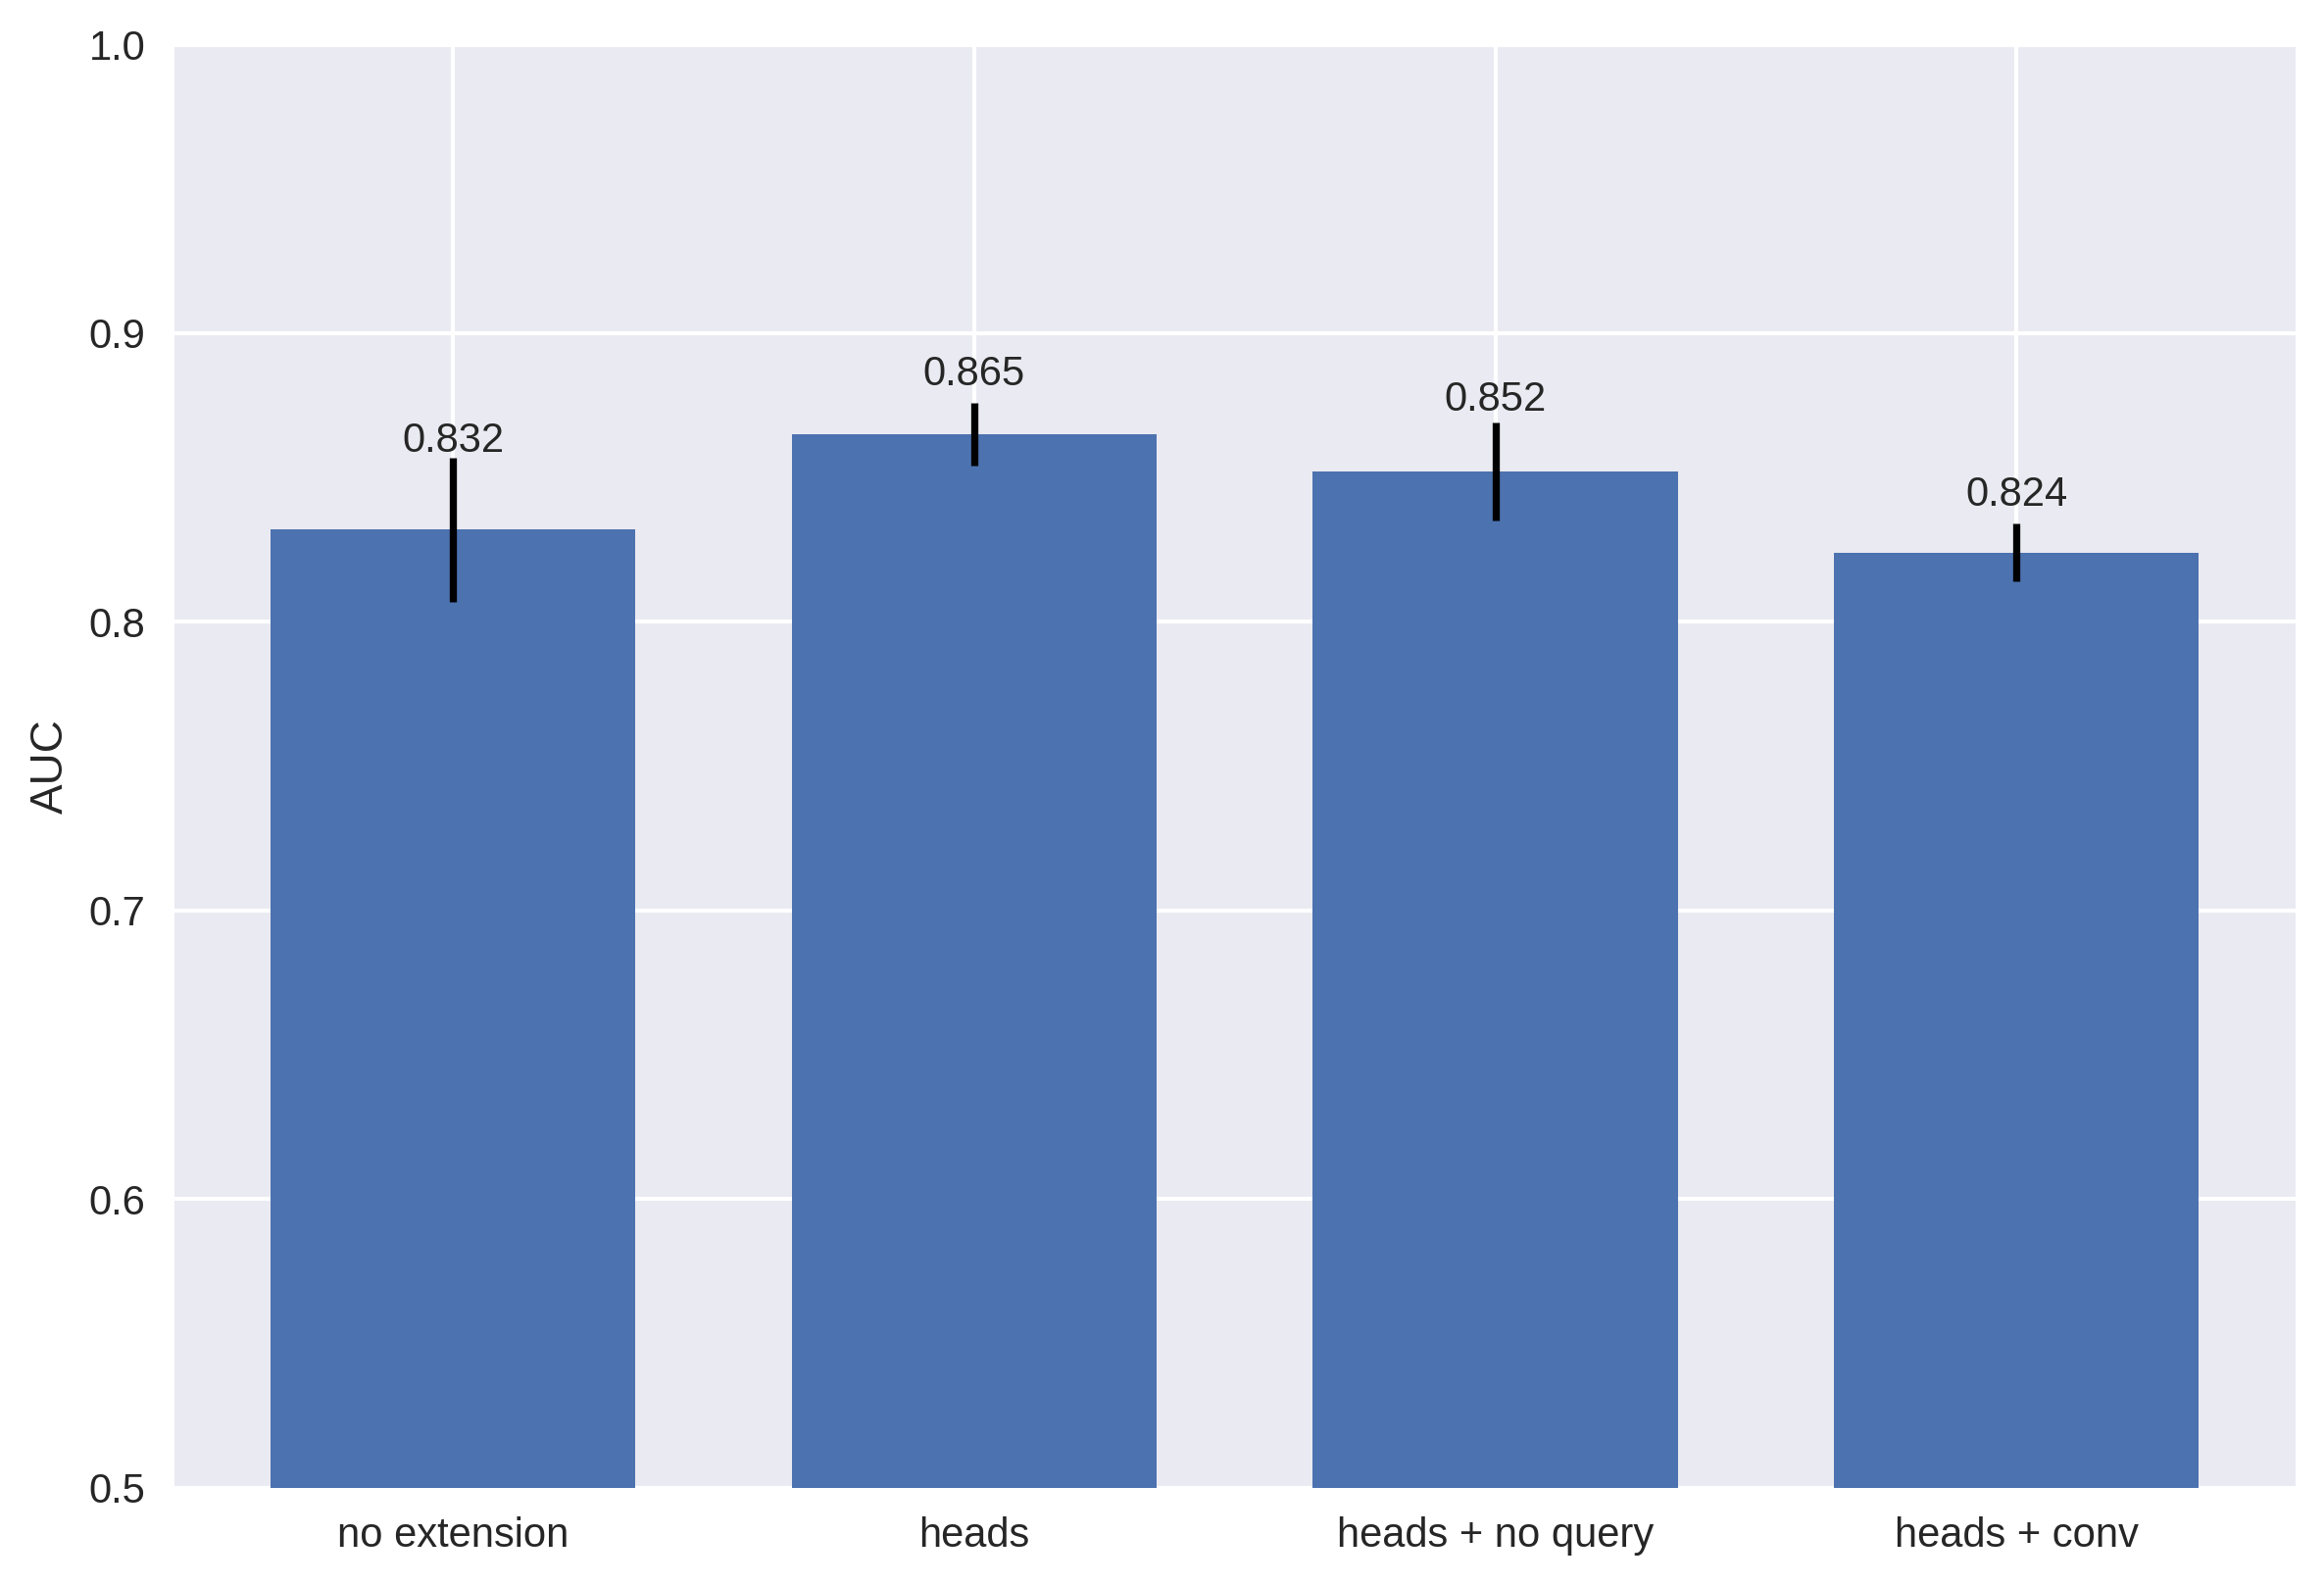
\includegraphics[width=1\textwidth]{../visualizations/ch5-results/attn_extension_barcharts.png} 
	\caption{Performance evaluation of the three extensions to the attention mechanism. We abbreviate the use of multiple attention heads as `heads', the removal of the query matrix as `no query' and the introduction of an additional convolution as `conv'. }
	\label{fig:attn_extension_barcharts}
\end{figure}


%compute average of conv training error: 0.9884710561726501 for conv + no query

%
%\begin{table}[h!]
%	\centering
%	\begin{tabular}{| c c c | c c | c} 
%		\hline
%		%   & configuration & & performance & \\
%		heads & no query & conv & $\mu$ & $\sigma$ \\
%		\hline
%		0 & 0 & 0 & 0.832 & 0.025 \\
%		0 & 0 & 1 & 0.860 & 0.021 \\
%		0 & 1 & 0 & 0.851 & 0.013 \\
%		0 & 1 & 1 & 0.818 & 0.019 \\
%		1 & 0 & 0 & \textbf{0.865} & 0.011 \\
%		1 & 0 & 1 & 0.824 & \textbf{0.010} \\
%		1 & 1 & 0 & 0.852 & 0.017 \\
%		1 & 1 & 1 & 0.846 & 0.017 \\
%		\hline
%	\end{tabular}
%	\caption{Results of evaluating the three additional attention extensions. $\mu$ denotes the average AUC across 9 experiments and $\sigma$ the respective standard deviation. 0 codes for the extension not being used, 1 codes for the extension being used. The extensions were abbreviated as follows: heads = multiple attention heads were used, no query = no conceptual query matrix was used, conv = an additional convolution operation was applied to the key and value matrices.
%	}
%	\label{table:attn_extensions}
%\end{table}
\subsubsection{Using multiple attention heads} \label{subsubsec:result_heads}
Using multiple attention heads leads to significantly improved performance and to significantly reduced variance between runs. Thus, the additional representational subspaces appear to improve performance and the ensemble model effect of multiple attention heads appear to reduce variance. No overfitting is observed, despite the number of model weights increasing from roughly 36,000 to 67,000 compared to the single attention head model. Due to the uniformly improved performance, we elect to incorporate multiple attention heads into RASC. 

%36361 -> 66861 

\subsubsection{Removing the query matrix}  % 56465 parameters
We observe slightly diminished performance upon removing the query matrix. The extra representational capacity afforded to RASC by having query matrices appears to improve its predictive power. Despite decreasing model size by roughly 10,000 parameters when removing the query matrices, we decide to not incorporate this adaption of the attention mechanism. 

%However, in initial experiments, the attention** mechanism performed significantly worse than the attention* mechanism. The extra representational capacity by having a query matrix seems to be important for performance. 
%In practice, this lead to a model about 10\% smaller. 
%In practice, this lead to an about 10\% smaller model.

%all 8 possible variations of combining them. Quantitative results are reported in Table \ref{table:attn_extensions}. 
%The overall best performing model uses multiple attention heads, but no other extensions. Using multiple attention heads appears to make the model perform consistently better than the baseline, except when paired with the convolution extension. On a closer look, this seems to be the result of the model overfitting to the dataset as shown in Figure [...]. %TODO
\subsubsection{Adding an extra convolution}
Adding an additional convolution operation to the attention mechanism, surprisingly leads to decreased performance, even comparing unfavorably to the baseline single-head attention model. This in contrast to \cite{ghentransformers} where this extension lead to very significant relative performance improvements. There are likely multiple factors contributing to these varying results:
% Reasons for why this extension did not work might be related to the use of a recurrent encoder as well as task differences:

\begin{figure}
	\centering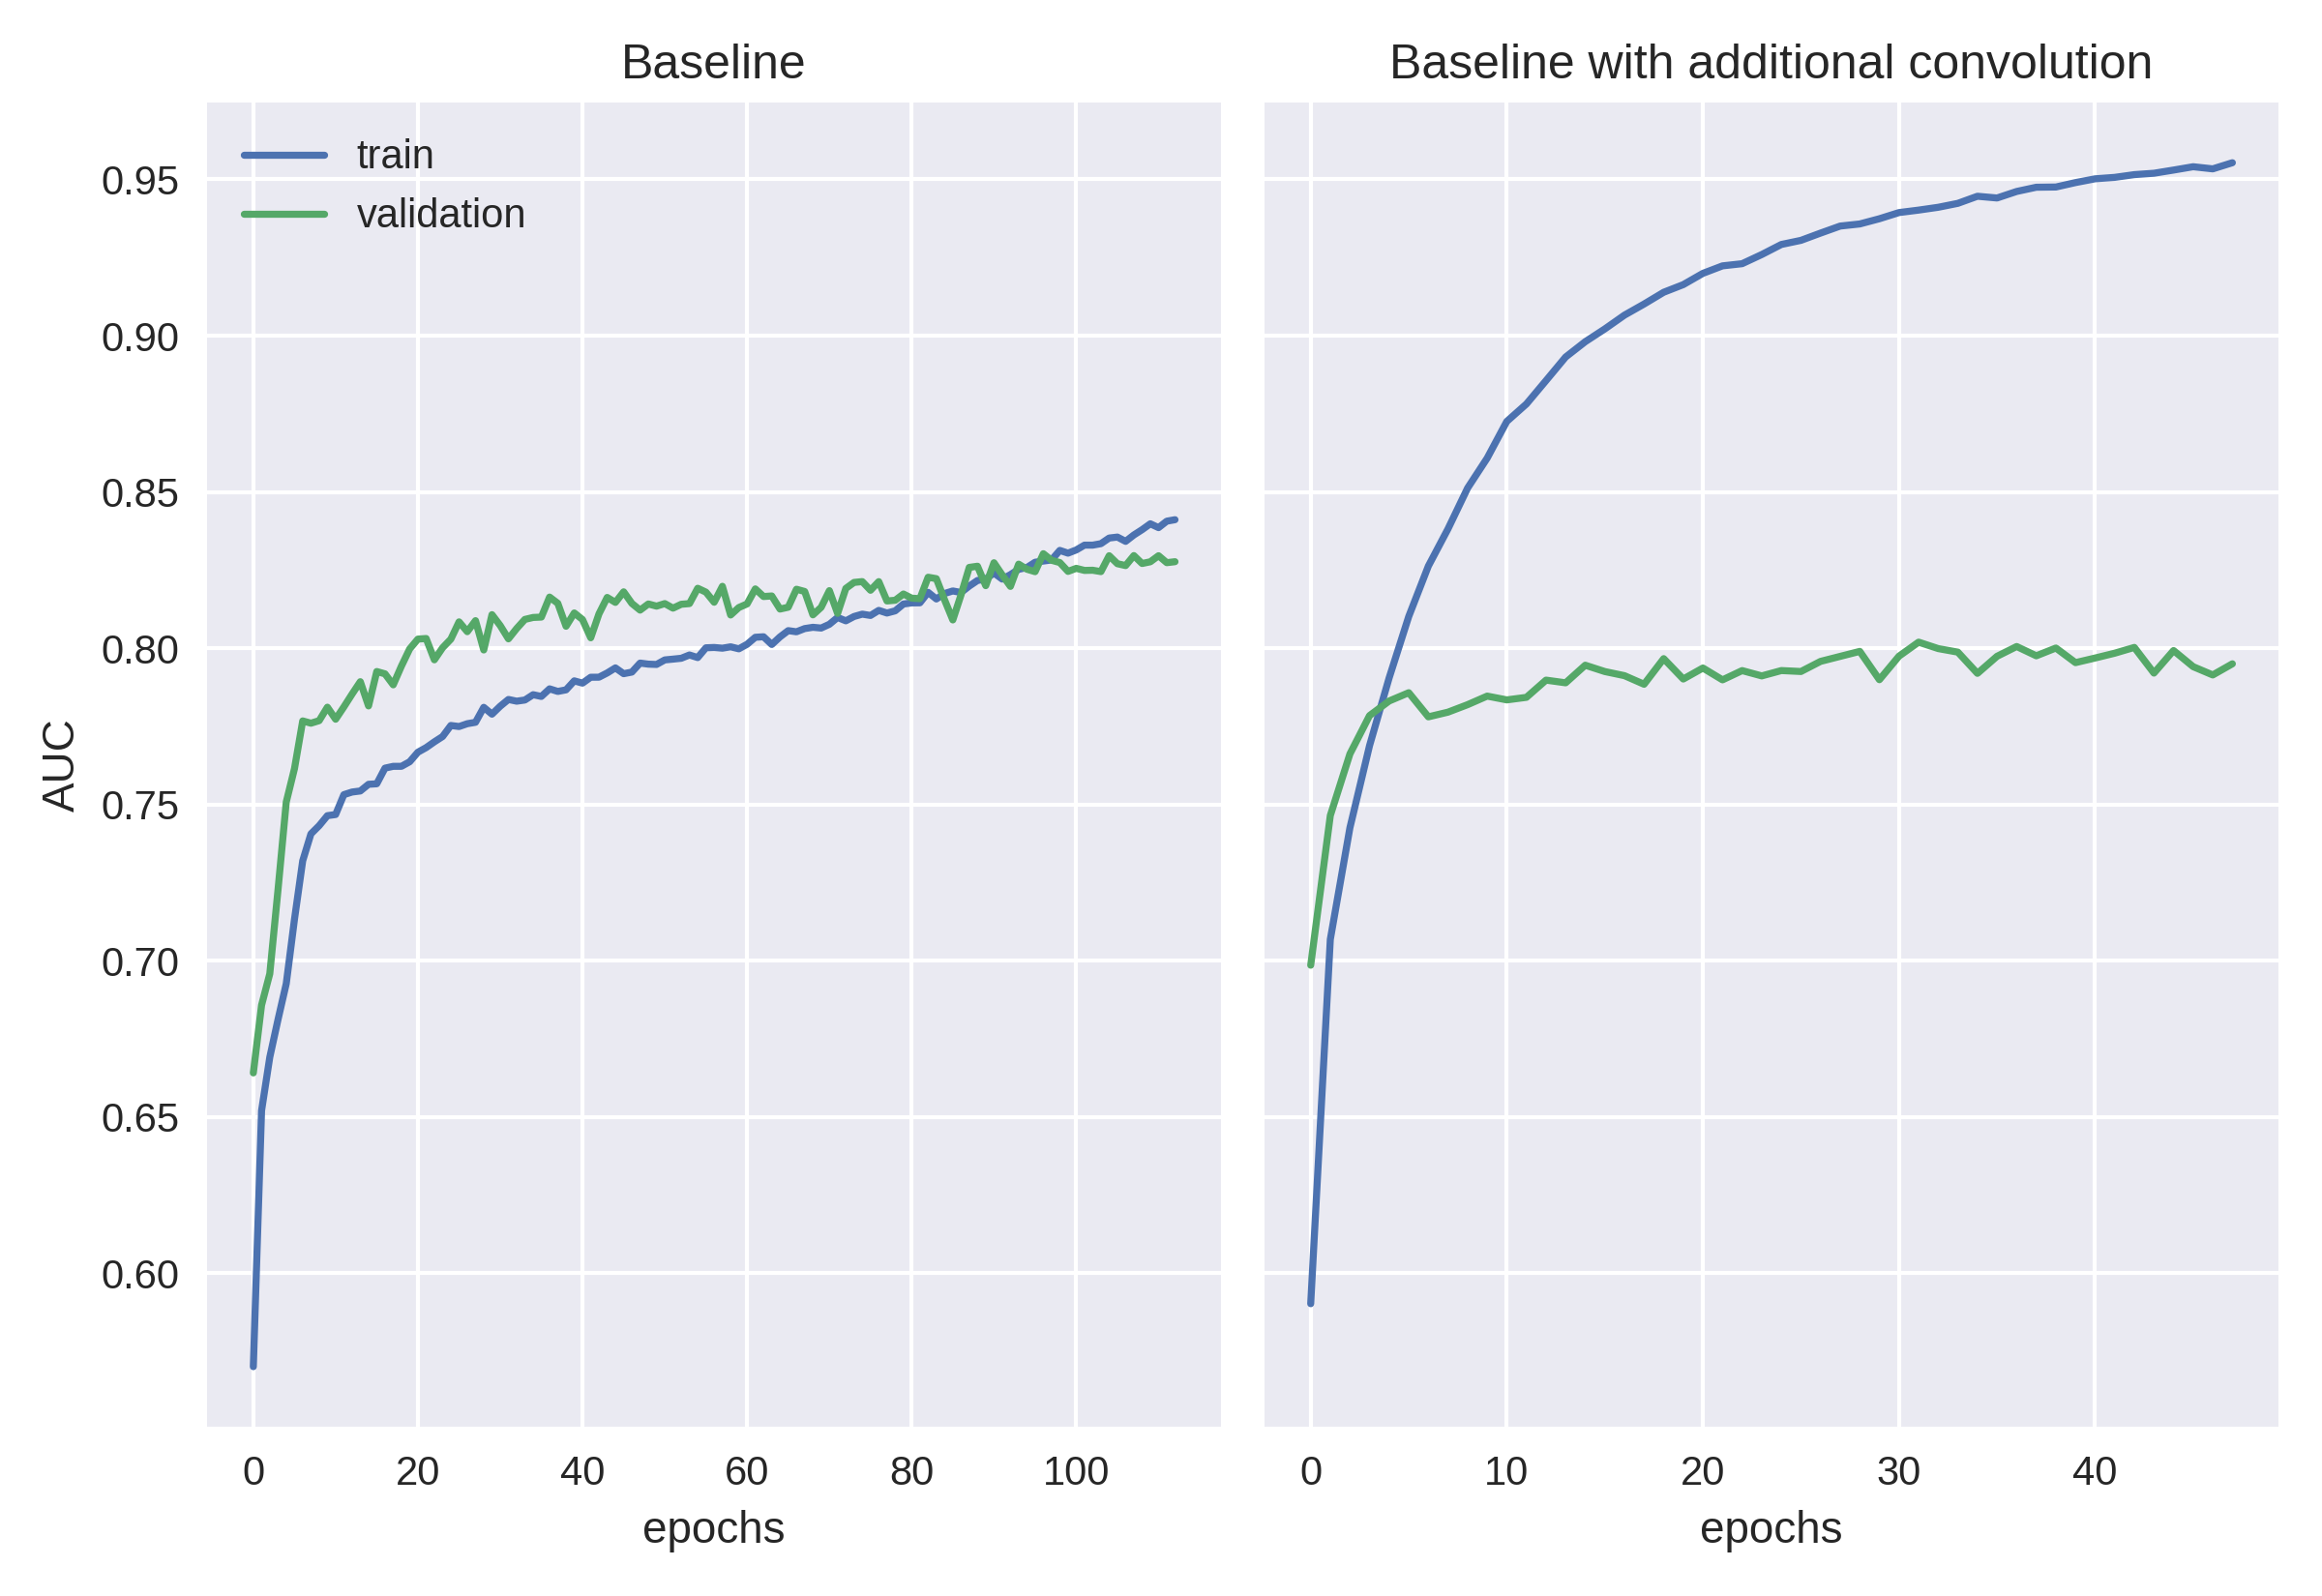
\includegraphics[width=1\textwidth]{../visualizations/ch5-results/training_curve_conv_heads2.png} 
	\caption{RASC overfits when the additional convolution operation is introduced into the attention heads. The baseline refers to RASC with multiple attention heads. }
	\label{fig:training_curve}
\end{figure}


\begin{enumerate}
	\item Although we process the input at single-nucleotide resolution, the use of a BiLSTM means that the encoder is aware of the nucleotides which precede and follow it. Therefore, the model can already encode information about the neighbouring nucleotides in the representation for a given nucleotide. This is in contrast to a Transformer model where the layers are non-recurrent and only work at single-nucleotide resolution. Thus, the convolutional layers likely give the model less additional modelling flexibility.
	\item In \cite{ghentransformers}, the task is full genome transcription start site annotation (so predicting where genes start). Therefore, their task occurs at the inter-gene level while our task occurs at the intra-gene level. This likely means that the motives \cite{ghentransformers}'s model has to consider generally span more nucleotides and granting the model more capacity to integrate information over multiple nucleotides is more crucial. 
	In contrast, granting RASC more capacity to integrate information over multiple nucleotides may not be necessary to identify the shorter motifs influencing splicing. 
%	TODO: biological plausibility of this?
%	In contrast, the comparably fine-grained working of RASC may be necessary for it to identify the shorter motifs which influence splicing. 
%	Thus, these differences likely also influenced the performance differences when using the convolutional attention layer extension in the different models.
	%		they: 3000 nucleotides, convolution filter of 7
	\item Furthermore, we observe overfitting when using this extension. The training curve in Figure \ref{fig:training_curve}
	showcases this behaviour. We observe overfitting despite using the same convolution across multiple heads, increasing the dropout probability in the attention heads, introducing additional batch normalization layers and limiting the convolution kernel size to 3 
	%TODO(see Table \ref{app:conv_tests} in the appendix for further results)
	. 
\end{enumerate}


In summary, we extend RASC with multiple attention heads. The results of RASC we report on the other datasets also use the model with multiple attention heads. 


%\subsection{MAJIQ with iPSCs differentiated to neurons (junctions)}
%haven't run experiments yet, not sure if results are interesting (but probably yes)\\
%due to training times, probably don't want to run these with cross-validation as that would take 15 hours+

\subsection{Sensitivity and specificity analysis}
\begin{figure}
	\centering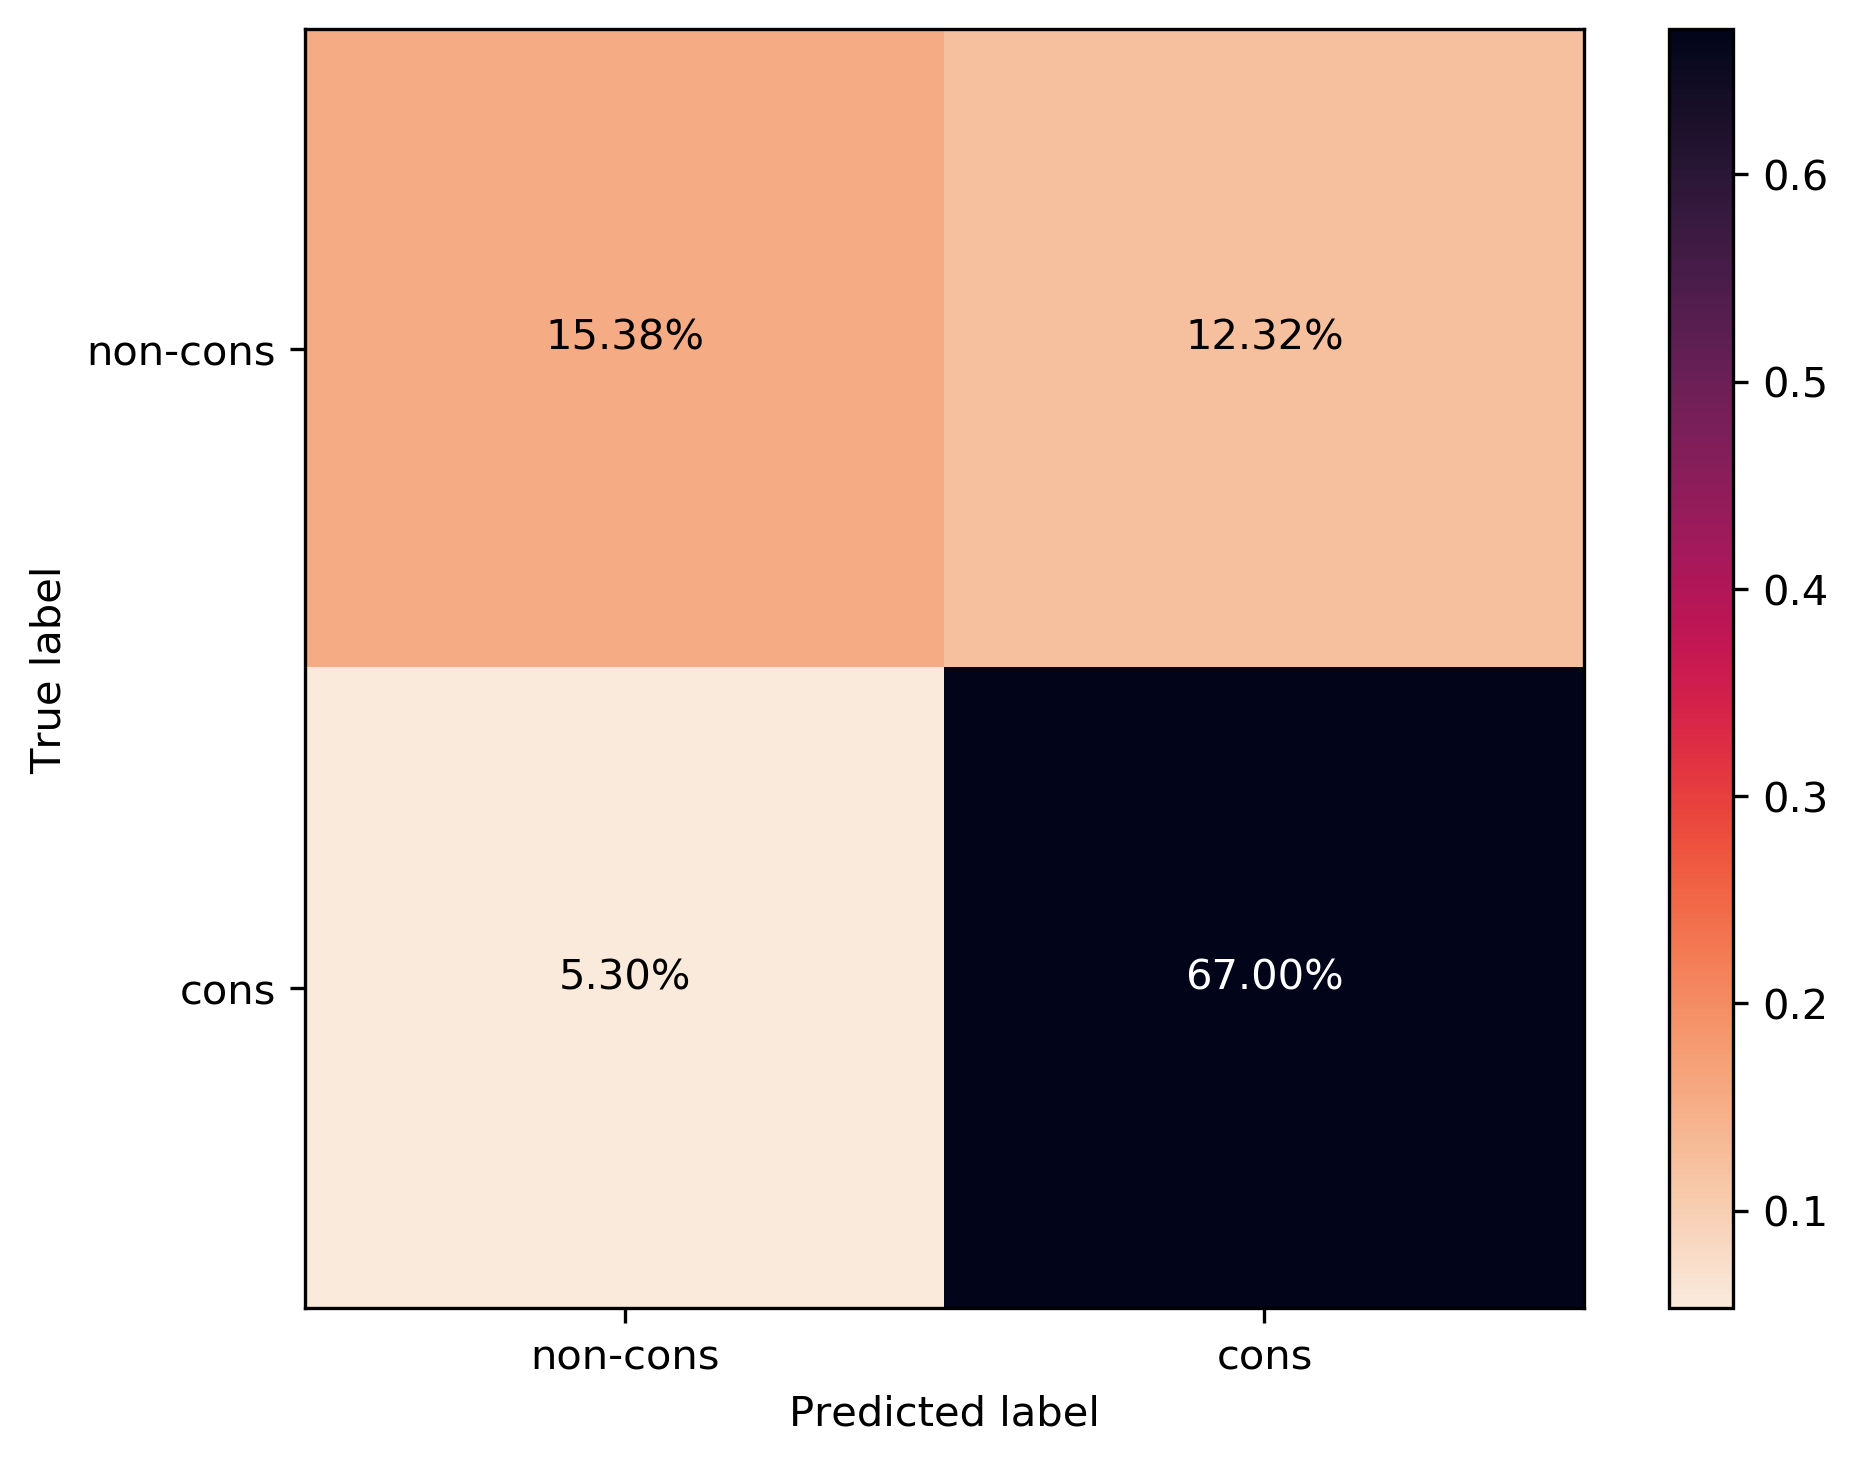
\includegraphics[width=0.7\textwidth]{../visualizations/ch5-results/confusion_matrix.png} 
	\caption{Confusion matrix from RASC on the neuron HipSci MAJIQ dataset. `cons' and `non-cons' respectively abbreviate constitutive and non-constitutive exons. }
	\label{fig:confusion_matrix}
\end{figure}

We present the confusion matrix for the binary classifier based on RASC in Figure \ref{fig:confusion_matrix}. The decision threshold which maximizes the F1 score was chosen resulting in a F1 score of 0.88 (for the negative class of constitutive exons). We observe comparatively few false positives, but many false negatives and correspondingly obtain a low sensitivity score of 0.56, but a high specificity score of 0.93. Thus, the classifier performs well at ruling in that an exon is alternatively spliced, but poorly at ruling that it isn't. This means the classifier is attractive for guiding the investigation of exons, where it wasn't previously known that they are alternatively spliced. This wouldn't be possible with a less specific classifier because further investigation relies on expensive wet-labs experiments for which the number of false positives need to be minimized. When employing RASC in practice, the decision threshold should be chosen such that the specificity is even higher (at the cost of further reduced sensitivity): a false positive rate of 5.3\% is still too high for wet lab experiments. Thus, we conclude that our classifier shows attractive properties, but would require further tuning before clinical use. 


\subsection{Cross-condition performance} \label{subsec:hipsci_ipsc_majiq}

\begin{figure}
	\centering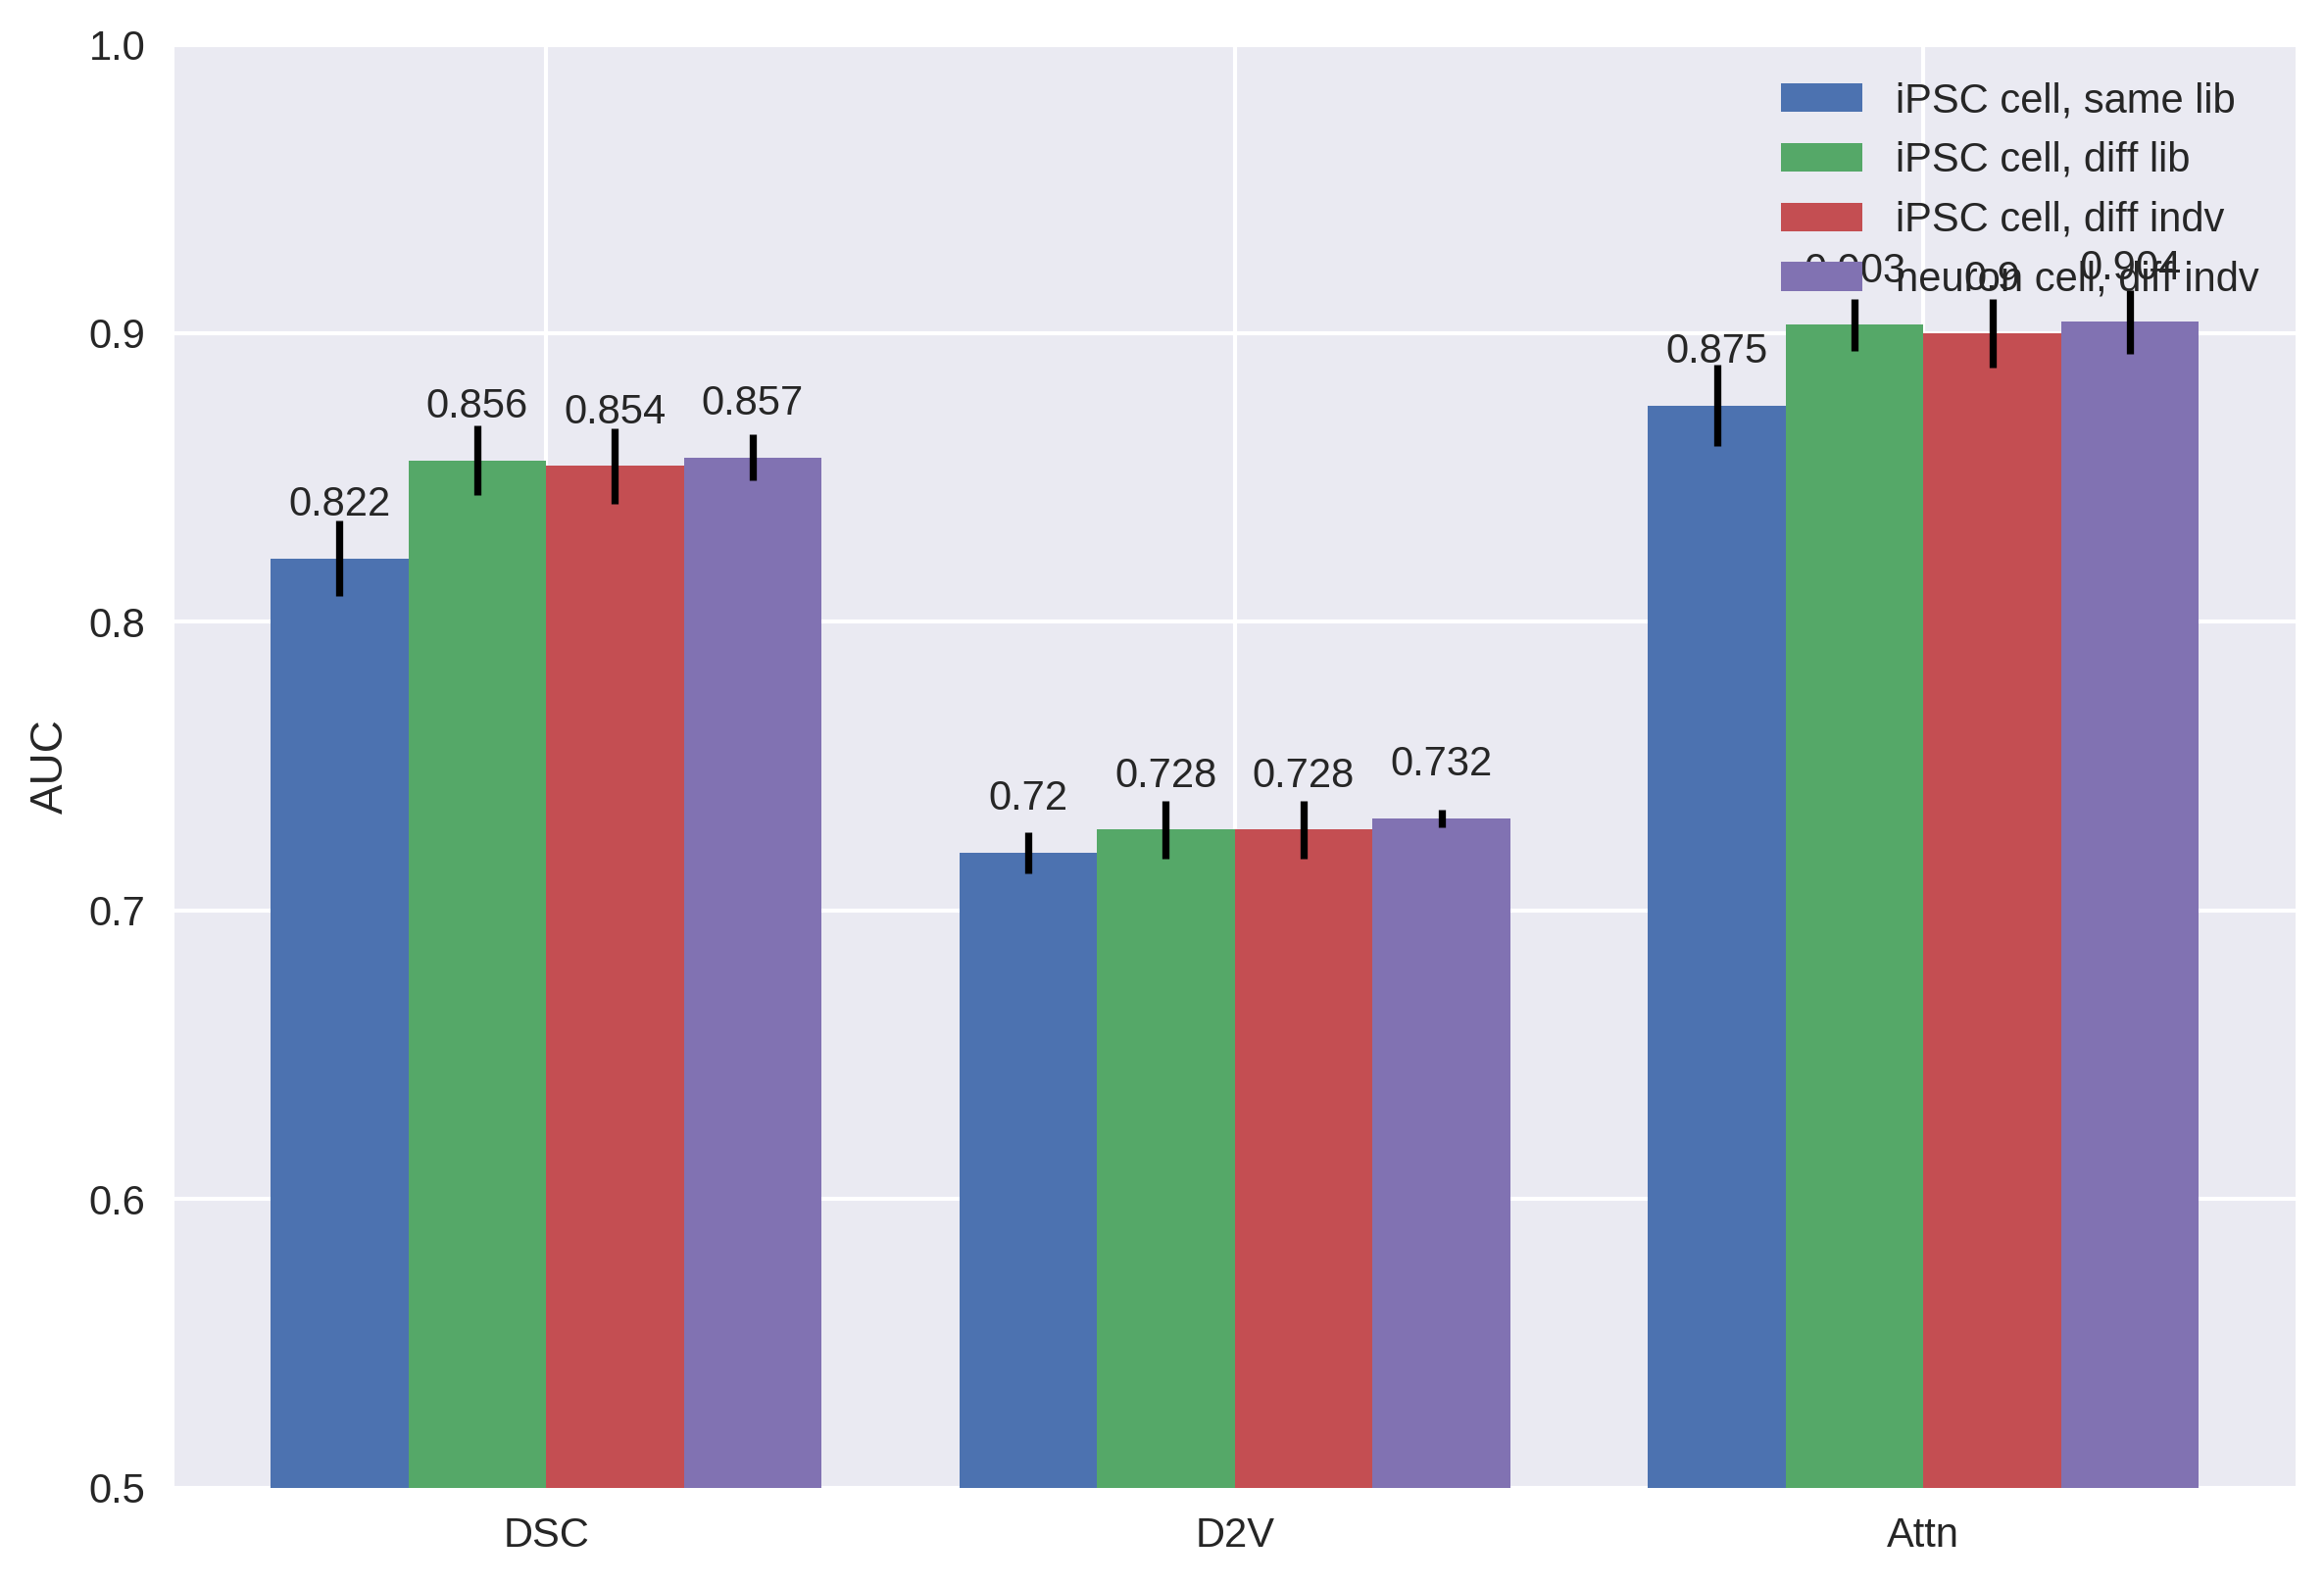
\includegraphics[width=0.7\textwidth]{../visualizations/ch5-results/majiq_comparison_barcharts.png} 
	\caption{Performance when training models on one HipSci dataset and testing on the same dataset as well as three others. Within the bars of one model, going further right means using a dataset which is less similar to the dataset the model was trained on (the left-most bar display performance when testing the model on the dataset it was trained on). `lib' refers to a library or biological sample from the same individual, `indv' refers to the indivdiual the sample was taken from, `diff' abbreviates different. `iPSC cell' refers to a dataset based on RNA-seq data from undifferentiated iPSC cells while `neuron cell' refers to iPSC cells differentiated to sensory neuron cells. }
	\label{fig:majiq_comparison_barcharts}
\end{figure}


We evaluate how well the models generalize when trained on a dataset derived from one individual and then tested on a dataset derived\footnote{When choosing the samples to evaluate on from the different datasets, care needs to be taken to avoid a subtle data leak: due to the specifics of MAJIQ, the original dataset and the dataset from the same individual but a different library share the consecutive exon training samples. This initially lead to the surprising observation that  it is better to train on a dataset different from the one the model is evaluated on. This issue is avoided by efficiently filtering all samples that are in the original training dataset from the three additional datasets through the use of a hash set.}
\begin{itemize}
	\item from the same individual, but a different library
	\item from a different individual, but the same cell type
	\item from a different individual from a different cell type
\end{itemize}


We visualize the results in Figure \ref{fig:majiq_comparison_barcharts}.
Unsurprisingly, performance drops slightly when a model is evaluated on a dataset different from the one it was trained on. Surprisingly, this performance drop does not directly correlate with the similarity to the original dataset: the least similar dataset from the different individual and different cell type performs best. 

However, to more seriously investigate how splicing differs between conditions, the capability of MAJIQ to quantify differential splicing should be taken advantage of. The best performing model, RASC, could be adapted such that it takes in an exon as well as two different conditions (e.g. via one-hot encoded tissues) and then predicts the change in splicing behaviour between the two conditions. 


%- constitutive exons are shared across all datasets
%- majiq builder builds up initial splice graph using all samples -- some confounding there for sure
%- for this sort of analysis, prediting differential splicing itself would be more apt
%
%cross-tissue comparison here with very low variance across tissues;\\
%seems like learned features are mostly tissue-invariant\\





% todo (maybe): actually evaluate other decision thresholds here

%              precision    recall  f1-score   support
%cons       0.74      0.56      0.64      1239
%non-cons       0.84      0.93      0.88      3234
%accuracy                           0.82      4473


% sensitivity: 0.56 -- ruling out alternatively spliced
% specificity: 0.93 -- ruling in alternative spliced
% f1 score: 0.88, precision: 0.845 (cons), recall (cons): 0.927











\subsection{Interpreting RASC} \label{subsubsec:attn_interpretation}


\begin{figure}
	\centering
	\makebox[0pt]{
		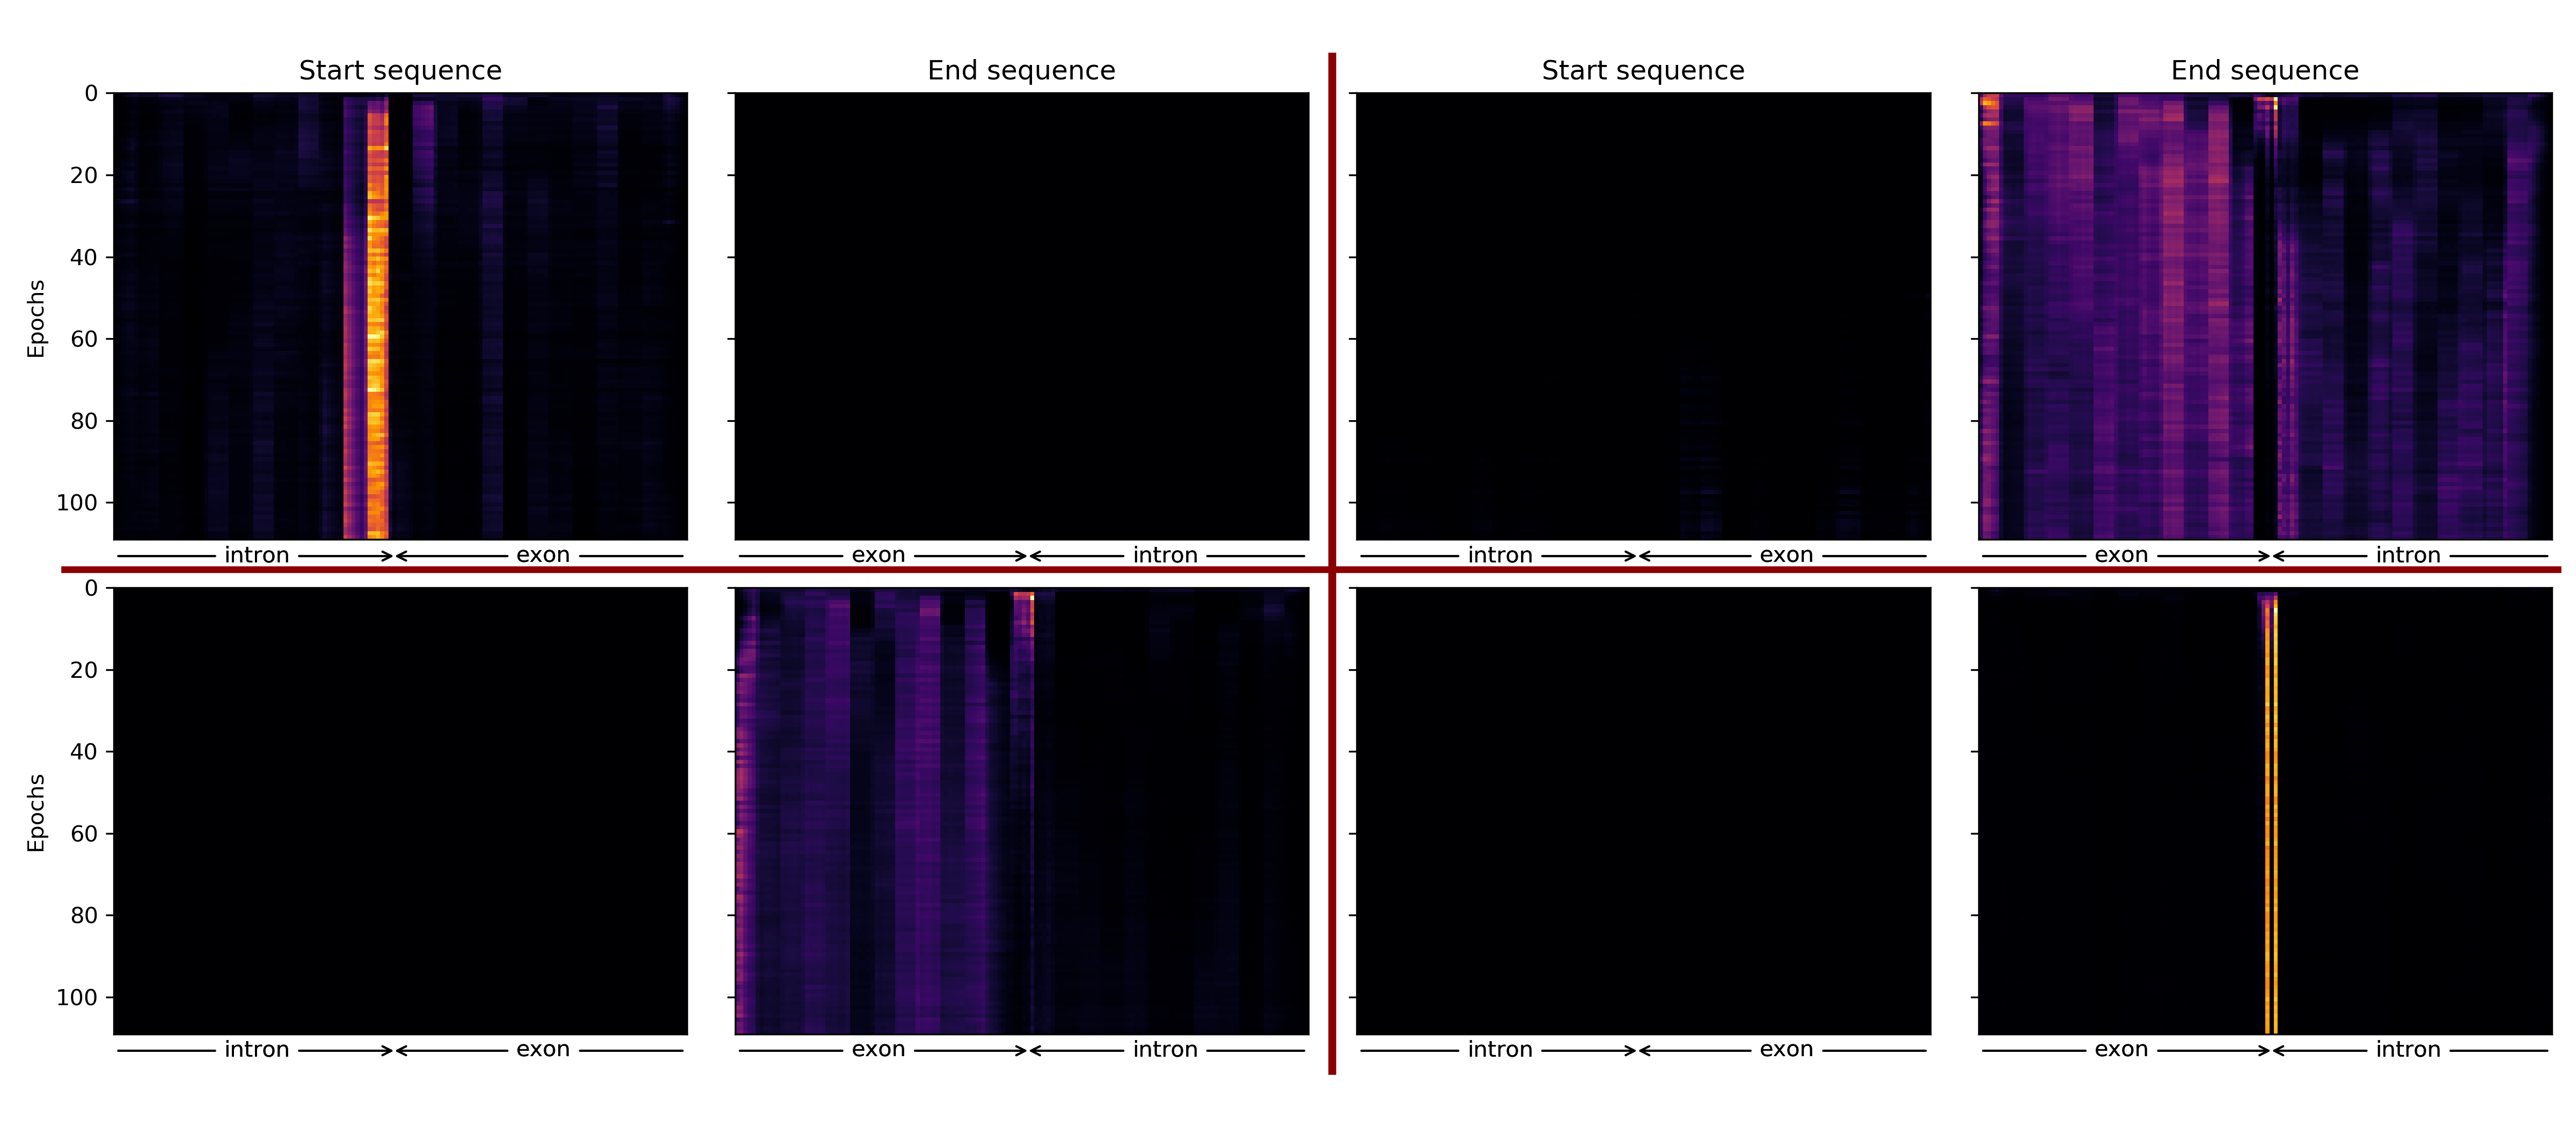
\includegraphics[width=1.3\textwidth]{../visualizations/ch5-results/attention_heatmap.png} 	}
	
		\caption{Each of the four quadrants shows the distribution of the attention weights for a single attention head. The distribution of attention weights is visualized via one heatmap for the start and one heatmap for end sequence, showing how the distribution of attention weights develops during training. The mean distribution of the attention weights over the test set is displayed.}
		\label{fig:attn_heatmap}

	
%	lines idea taken from https://discourse.matplotlib.org/t/horizontal-and-vertical-lines-between-subplots/13540 or powerpoint, https://stackoverflow.com/questions/26084231/draw-a-separator-or-lines-between-subplots?rq=1
\end{figure}

%We visualize to what parts of the input sequence RASC pays attention to in \ref{fig:attn_distribution}. 

%graphics in this section:\\
%- 4x2 heatmaps of mean attention over epochs of all four attention heads\\
%- 1 barchart of final mean attention over mean of all attention heads\\
%- 1+ barcharts for analyzing specific exons

%heatmap analysis:
%\begin{itemize}
%	\item Different attention heads focus on different things, although some overlap
%	\item attention rarely extremely focussed, but honestly can't really tell on this picture
%\end{itemize}

\subsubsection{Heads focus on a single sequence} 
When using a single attention head, the head needs to split its conceptual `focus' over the start and end input sequences. This is not the case for multiple attention heads: here single heads may focus on only one sequence as long as there is at least one attention head which also pays attention to the information in the other sequence. We observe exactly this behaviour in Figure \ref{fig:attention_heatmap}: one of the attention head attends purely to the start sequence and all other attention heads attend purely to the end sequence. Across the 9 cross-validation runs, single attention heads only split their `focus' 7 out of 36 times. None of the trained models only ever pay attention to only a single sequence. This reassures us that the dataset isn't biased such that the model only needs to take information from one sequence into account. 

The sequence which an attention head focusses on generally does not change after the first 5 epochs. Similar observation, that the role of attention heads is decided very early on in training, have also been made in the context of NLP \cite{sixteenheads}.

\subsubsection{What does the model pay attention to?}

\begin{figure}
	\centering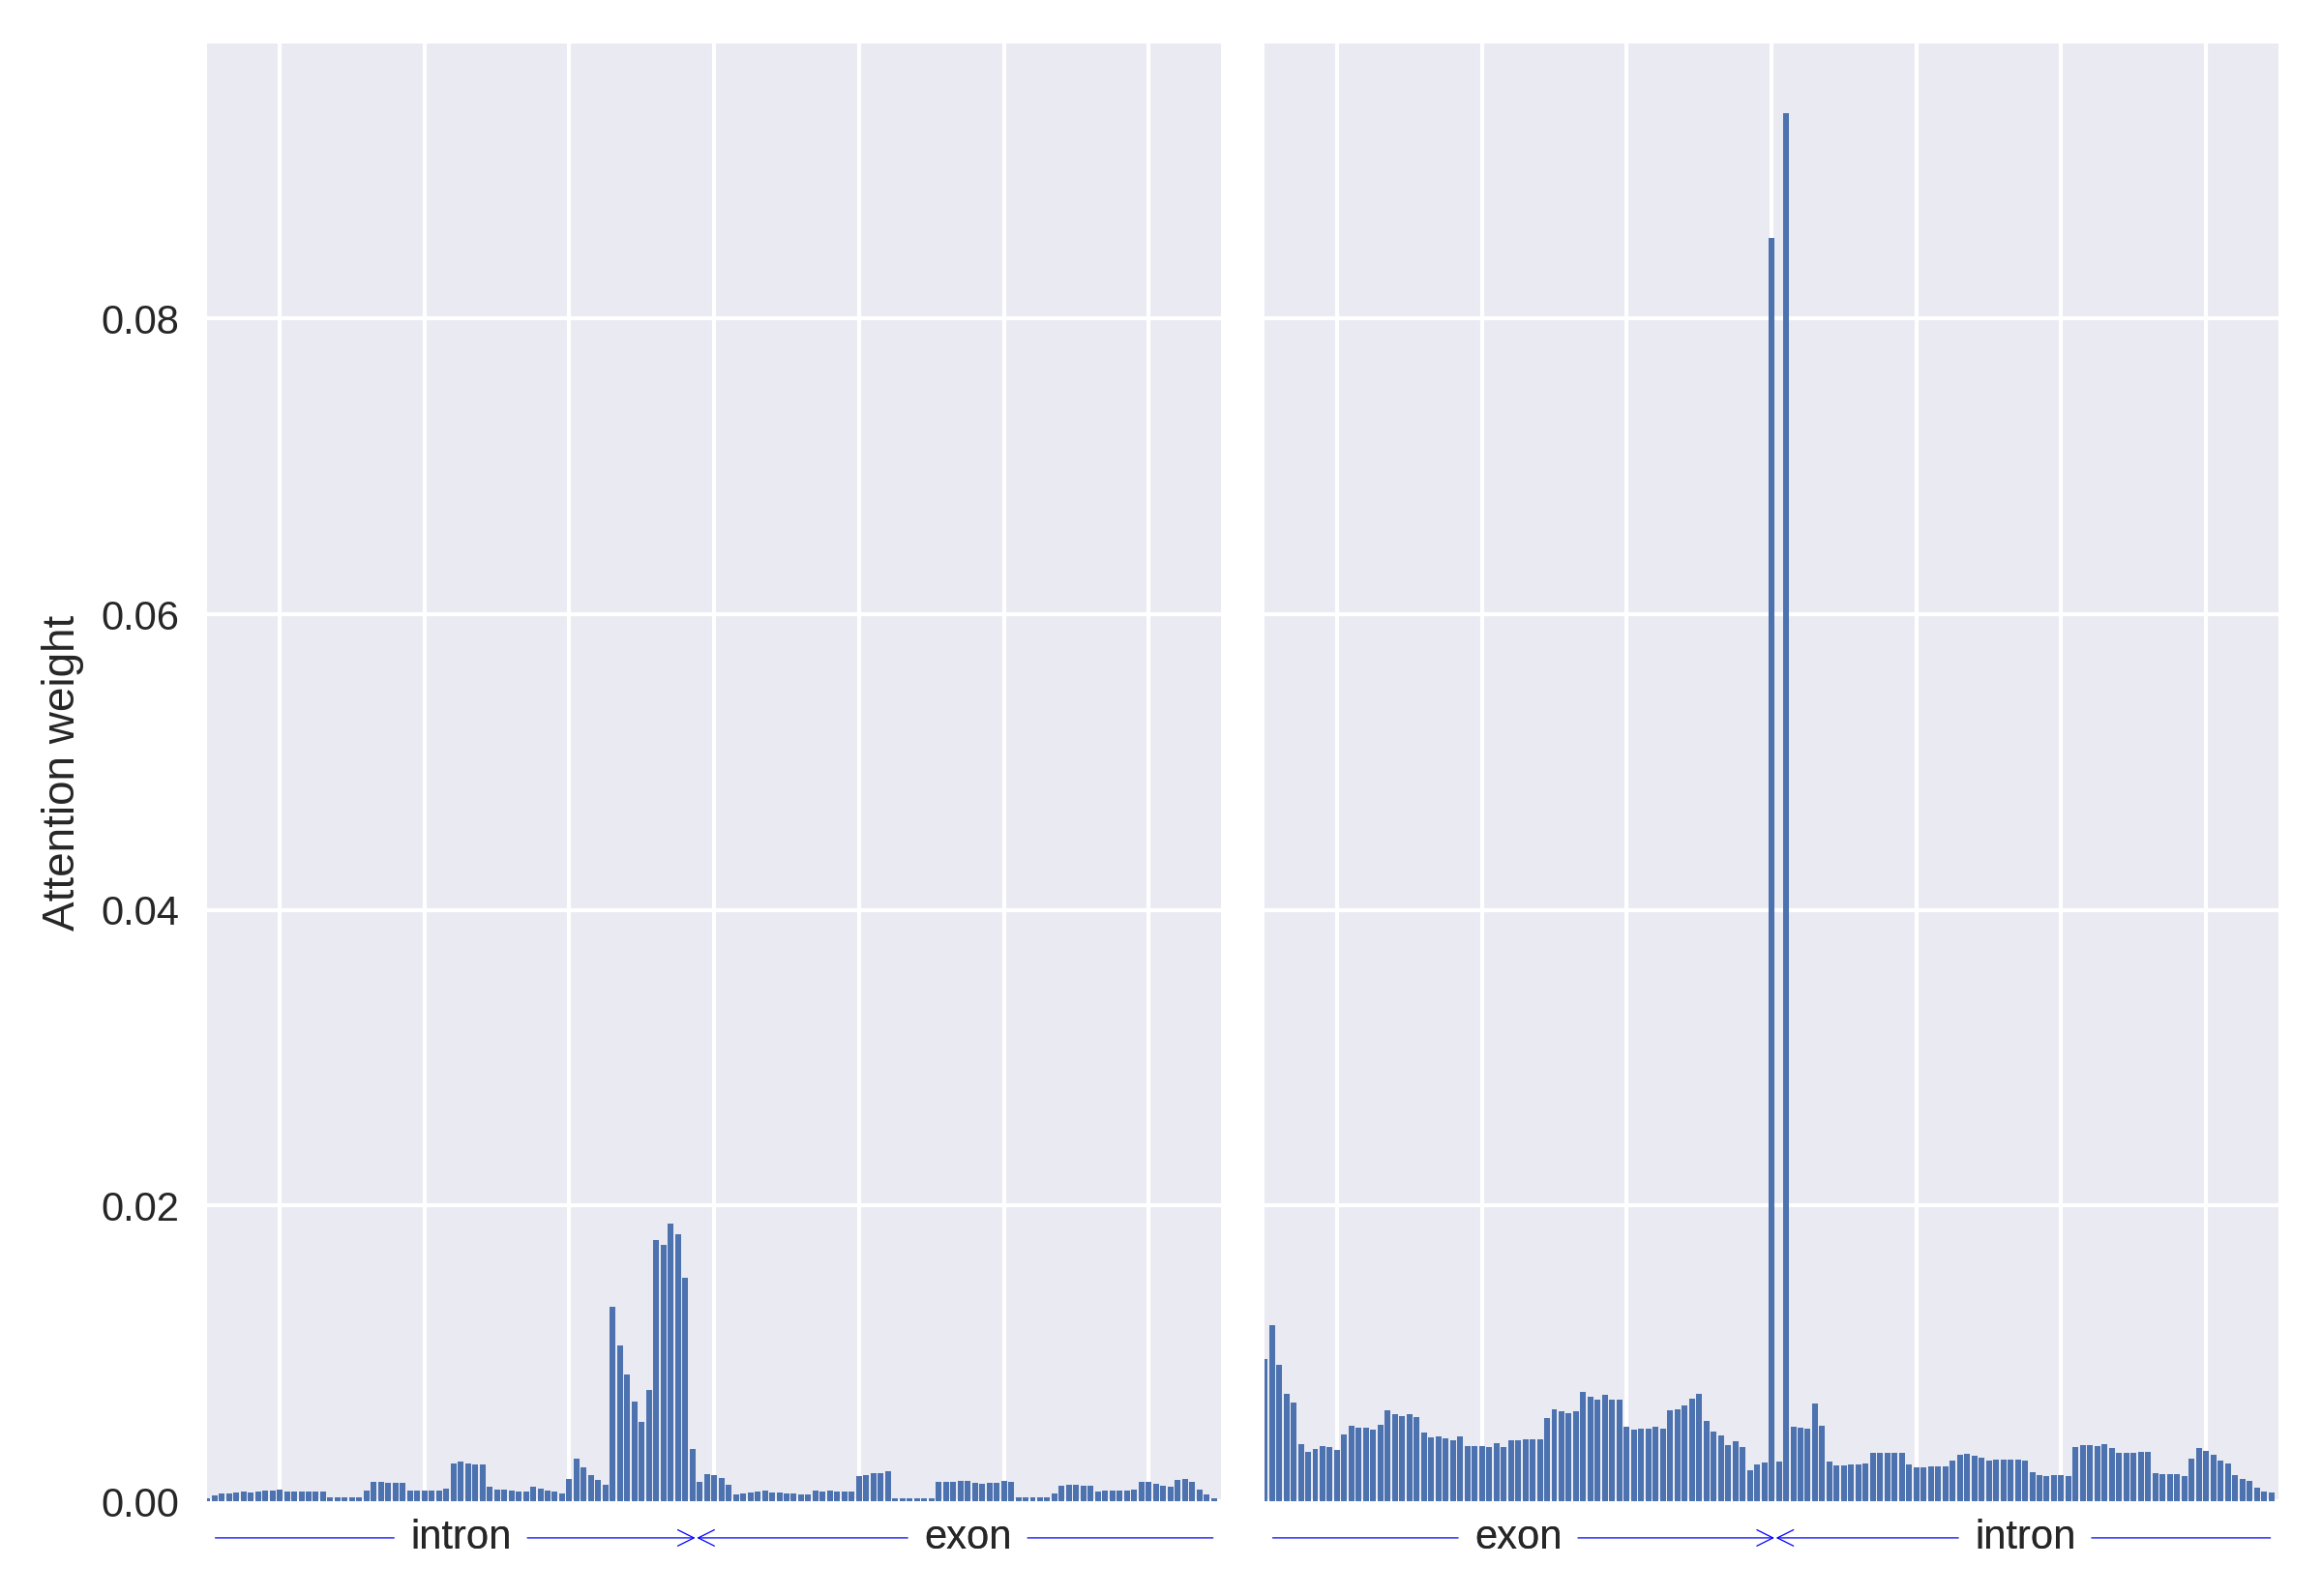
\includegraphics[width=1\textwidth]{../visualizations/ch5-results/mean_attention_barchart.png} 
	\caption{Mean attention weights averaged over all test samples and all four attention heads. }
	\label{fig:mean_attn}
\end{figure}
Averaging the attention weights over all heads at the end of training, we visualized the most attended to parts of the input sequence in \ref{fig:mean_attn}.
%Figure \ref{fig:mean_attn} shows what part of the input sequence RASC commonly attends to. 
Clearly, motifs directly around the exon start and exon end are the most attended to. 

%TODO now this is a job for Liz and Wil
The bar chart suggests that more total attention is paid to the end, rather than the start sequence. However, this pattern is reversed for other runs of the models and likely just a sequence of three attention focusing on the end sequence in this particular training run. Additionally, note that the weighting of the outputs of the different attention heads by the unifying matrix $W^O$ is not displayed. 


%\begin{figure}
%	\centering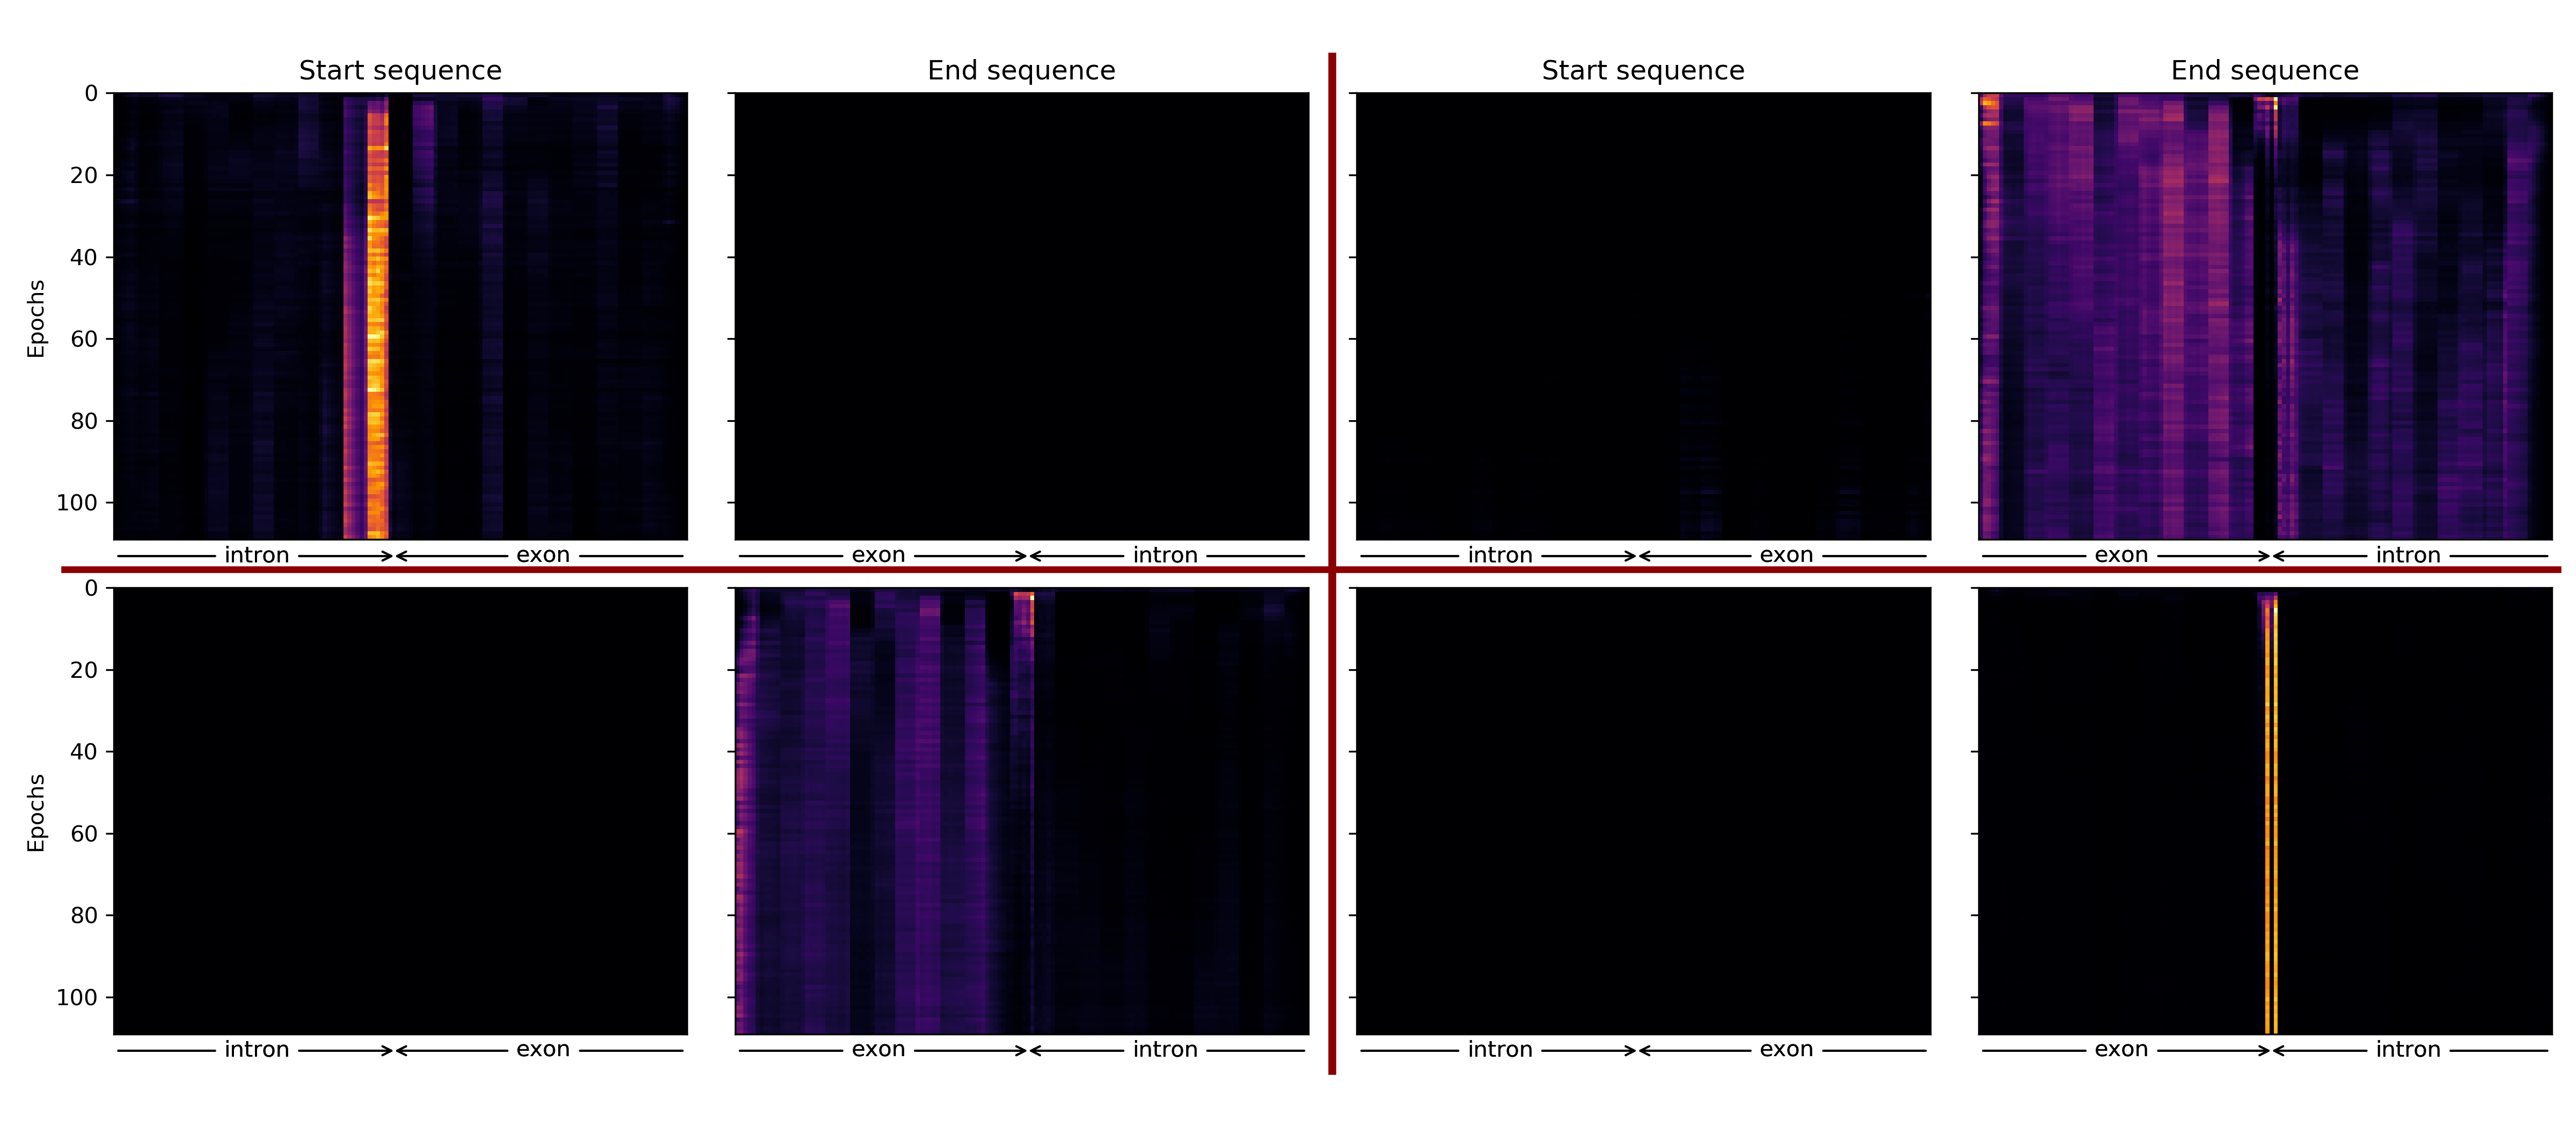
\includegraphics[width=1\textwidth]{../visualizations/ch5-results/attention_heatmap.png} 
%	\caption{Development of attention during training. }
%	\label{fig:attn_heatmap}
%\end{figure}






%attention distribution, proper:
%run id | distribution of heads
%0 | end/end/end/start
%1 | start/end/end/end
%2 | start/start/end/end
%3 | start/start/start/start but then mixed/mixed/mixed/mixed
%4 | end/start/end/start
%5 | start/start/start/mixed
%6 | start/end/start/start (tiny bit mixed 0.8)
%7 | start/end/start/start
%8 | end/mixed/end/mixed (from end/end/end/end at the beginning, switch after like 60 epochs)



\subsection{PSI Regression} \label{subsubsec:psi_regression}
After having achieved a good level of performance on the classification task, we turn to the regression task. We train the models on the sensory neuron cell HipSci MAJIQ dataset and give the results in Table \ref{table:psi_regression}. 


\begin{table}
	\centering
	\begin{tabular}{ c c c c c c c} 
		\hline
		Model & AllPSI &  LowPSI &  HighPSI \\
		\hline
		DSC	&	0.244   $\pm$	0.036	&	0.340	$\pm$	0.039	&	-77.980	$\pm$	13.631\\
		D2V	&	0.120	$\pm$	0.009	&	0.155	$\pm$	0.010	&	-57.523	$\pm$	2.771\\
		RASC	&	\textbf{0.486}	$\pm$	0.067	&	\textbf{0.595}	$\pm$	0.074	&	\textbf{-25.470}	$\pm$	5.717\\
		\hline
	\end{tabular}
	\caption{Mean $R^2$ for PSI regression task on sensory neuron cell HipSci MAJIQ dataset.  $\pm$ denotes standard deviation. 
	}
	\label{table:psi_regression}
\end{table}


The results show that the models still fail to explain a lot of the variation in the PSI value: no model is able to explain even half of it. 
As on the classification tasks, RASC outperforms the other models by a wide margin and all models are significantly worse on explaining the variance for highly included, rather than rarely to moderately included, non-constitutive exons. The latter observation is particularly pronounced: the $R^2$ score of all models is below 0, showing that they fail to explain the variance even as well as the baseline model whom consistently predicts the mean. Thus, we take these results as indication that the current Splicing Codes can still be significantly improved. 



%We generally observe poor to middling performance: DSC and D2V don't beat the baseline model with . Again, RASC outperforms the other models by a wide margin. 
%Like in the exon classification task, all models perform significantly worse on highly than on rarely to moderately included non-constitutive exons. 

\begin{table}
	\centering
	\begin{tabular}{ l c c c c c c} 
		\hline
		Model & Performance \\
		\hline
		BNN-UDC \cite{jha} & 0.220\\
		BNN-LMH \cite{jha}& 0.368\\
		DNN-PSI \cite{jha} & 0.434\\
		D2V \cite{d2vsplicing} & 0.594\\
		W2V \cite{d2vsplicing} & \textbf{0.680}\\
		\hline
	\end{tabular}
	\caption{Mean $R^2$ over 5 tissues for PSI regression task on mouse dataset as reported by \cite{d2vsplicing}. 
	}
	\label{table:ieee_regression}
\end{table}

%what percentage are non highly included ones? 
To further compare our model to other work, we repeat the main results from \cite{d2vsplicing} in Table \ref{table:ieee_regression}. \cite{d2vsplicing} used a dataset derived from mouse sequencing data, originally from \cite{jha}. On this dataset, D2V is the second-best performing model, only moderately outperformed by a more finer-grained word2vec model (denoted W2V). Nonetheless, D2V significantly outperforms all other models from the literature it was compared to. Note that the models evaluated by \cite{d2vsplicing} comprise all of splicing codes from the last 5 years which we are aware of. However, D2V is significantly outperformed by RASC on our dataset. This indicates that RASC would compare very favorably against all models also evaluated in \cite{d2vsplicing}. 

%TODO: indirect evaluaton -> 5 models
%https://blog.minitab.com/blog/adventures-in-statistics-2/regression-analysis-how-do-i-interpret-r-squared-and-assess-the-goodness-of-fit

We also observe that the $R^2$ values reported by \cite{d2vsplicing} are significantly higher: the best performing model W2V is able to explain nearly 70\% of the variance. We consider multiple possible explanations for this: 
\begin{itemize}
	\item Splicing behaviour on the mouse dataset is easier to predict because of data processing differences. Like our work, \cite{d2vsplicing} use MAJIQ for data processing. While they don't explicitly state the version of MAJIQ they used, MAJIQ has received various updates since their publication. These updates include improvements to the splicing detection algorithm which could affect the outcome of data processing. 
	\item Splicing behaviour on the mouse dataset is easier to predict because of dataset composition differences. The mouse dataset only includes cassette exons, while our dataset also includes constitutive non-cassette exons. Since splicing motifs between cassette and non-cassette exons likely differ, the learning task of our models could be more challenging since they have to learn to recognize both. As a counter point, the mouse dataset only contains 10,000 training samples which might be too few samples to train our models.

	

	\item Splicing behaviour on the mouse dataset is easier to predict because of different model inputs. \cite{d2vsplicing}'s models D2V and W2V take 300 nucleotides, instead of 70 nucleotides, before and after the cassette exon start and end sites as input. In addition, they are also given analogue 600 nucleotide windows around the exon start and end sites directly flanking the cassette exon. In total their models are given 2400 nucleotides as input, while we give our models a total of 280 nucleotides as input. Widening the input context may help to equalize the performance between the mouse dataset and our dataset. 
	\item Splicing behaviour on the mouse dataset is easier to predict because it is less complex. Increased relative prevalence in exon skipping has been observed for more complex eukaryotic organisms \cite{splicing_current_perspectives}, giving plausibility to this explanation. However, we observed nearly no cross-tissue performance differences between tissues, when cross-tissue splicing behaviour is also known to vary \cite{crosstissuesplicing}. This hypothesis is incredibly challenging to evaluate, as there are many dimensions to splicing and no universal measure for splicing complexity (nor likely ever will be). However, due to the other possible explanations we explored and due to the low cross-tissue performance differences we observed, we evaluate it as unlikely.
	
	%	Progress towards evaluating this hypothesis could be taken by evaluating our models on the mouse dataset and seeing whether . However, the the mouse dataset is not publicly available and we are predominantly interested in splicing in humans due to its practical applicability. Thus, we do not pursue this avenue. 
\end{itemize}

While most of these possible explanations are difficult to falsify, increasing the amount of sequence information given to the models is a simple to implement and promising avenue of research which we leave to future work. 










%for destruction of EST the following may be interesting: Quantitative comparison of EST libraries requires compensation for systematic biases in cDNA generation

%perhaps mention how older psi regression methods used mouse data but we want human data and that is why we can't use their datasets


%motivation for why classification task was chose and not regression:
%older methods used mouse data
%we reimplement models from regression
%we start off with classification and then move on to regression once we get good enough perforamnce as regression is more challenging
%reasonable to assume that progress in one will also lead to progress in the other

%observation that best performing datasets contain the most samples



